\documentclass[fleqn,10pt]{wlscirep}
\usepackage[utf8]{inputenc}
\usepackage[T1]{fontenc}

\usepackage{cite}
\usepackage{amsmath,amssymb,amsfonts}

%\usepackage{tabularx,booktabs}
\usepackage{algorithmic}
\usepackage{multirow, graphicx}
\usepackage{subcaption}
\usepackage{textcomp}
\usepackage{upgreek}
\usepackage{longtable, booktabs}
% \usepackage{arydshln}
\usepackage{afterpage}  % load the afterpage package
\usepackage{color, soul}
\usepackage{lineno}
\linenumbers


%%% HELPER CODE FOR DEALING WITH EXTERNAL REFERENCES
\usepackage{xr}
\makeatletter
\newcommand*{\addFileDependency}[1]{
  \typeout{(#1)}
  \@addtofilelist{#1}
  \IfFileExists{#1}{}{\typeout{No file #1.}}
}
\makeatother

\newcommand*{\myexternaldocument}[1]{
    \externaldocument{#1}
    \addFileDependency{#1.tex}
    \addFileDependency{#1.aux}
}

%
\usepackage{csvsimple}
\usepackage{xstring} % defines \StrDel

\newenvironment{hlbreakable}%
{\color{brown}}%
{}



\usepackage{acro}


\usepackage{pifont}
\newcommand{\cross}{\ding{61} }%
\newcommand{\asterisk}{\ding{87} }%


%\def\BibTeX{{\rm B\kern-.05em{\sc i\kern-.025em b}\kern-.08em
%		T\kern-.1667em\lower.7ex\hbox{E}\kern-.125emX}}
%\markboth{\journalname, VOL. XX, NO. XX, XXXX 2020}
%{E. Finnegan \MakeLowercase{\textit{et al.}}: }

\DeclareMathOperator*{\argmin}{argmin} % thin space, limits underneath in displays

\graphicspath{{figures/}}
%\RequirePackage{subfig}
\RequirePackage[none]{hyphenat}
\RequirePackage{siunitx}

\RequirePackage{lipsum}
\RequirePackage{xifthen}

%To be able to hide a column in table
\usepackage{array}
\newcolumntype{H}{>{\setbox0=\hbox\bgroup}c<{\egroup}@{}}

\definecolor{TodoTitleColour}{rgb}{0.8,0,0}
\definecolor{TodoSampleColour}{rgb}{0.4,0,0}

% Usage: [number_of_paragraphs]{message}
\newcommand{\todo}[2][]{ 
	\textcolor{TodoTitleColour}{@TODO: #2}
	\ifthenelse{\isempty{#1}}
	{}
	{\textcolor{TodoSampleColour}{... SAMPLE TEXT: \lipsum[#1]}}
}



\makeatletter
\def\thickhline{%
  \noalign{\ifnum0=`}\fi\hrule \@height \thickarrayrulewidth \futurelet
   \reserved@a\@xthickhline}
\def\@xthickhline{\ifx\reserved@a\thickhline
               \vskip\doublerulesep
               \vskip-\thickarrayrulewidth
             \fi
      \ifnum0=`{\fi}}
\makeatother

\newlength{\thickarrayrulewidth}
\setlength{\thickarrayrulewidth}{5\arrayrulewidth}


%% Acronyms

\DeclareAcronym{tpr}{
  short=TPR,
  long=total peripheral reistance,
}
\DeclareAcronym{bp}{
  short=BP,
  long=blood pressure,
}
\DeclareAcronym{sbp}{
  short=SBP,
  long=systolic blood pressure,
}
\DeclareAcronym{dbp}{
  short=DBP,
  long=diastolic blood pressure,
}
\DeclareAcronym{map}{
  short=MAP,
  long=mean arterial blood pressure,
}
\DeclareAcronym{pe}{
  short=PE,
  long=phenylephrine,
}
\DeclareAcronym{pat}{
  short=PAT,
  long=pulse arrival time,
}
\DeclareAcronym{sqi}{
  short=SQI,
  long=signal quality index,
}
\DeclareAcronym{iqr}{
  short=IQR,
  long=interquartile range,
}
\DeclareAcronym{rmse}{
  short=RMSE,
  long=root mean squared error,
}
\DeclareAcronym{mae}{
  short=MAE,
  long=mean absolute error,
}
\DeclareAcronym{rho_p}{
  short=$\rho_p$,
  long=Pearson's correlation coefficient,
}
\DeclareAcronym{bmi}{
  short=BMI,
  long=body mass index,
}
%%


%
% Reference to the labels and numbers of chapter, section, figures, ...
%

\RequirePackage[noabbrev]{cleveref}
% Default folder for figures
\graphicspath{{figures/}}

\title{Features from the photoplethysmogram and the electrocardiogram for estimating changes in blood pressure}

\author[1,*]{Eoin Finnegan}
\author[1]{Shaun Davidson}
\author[1,2,3]{Mirae Harford}
\author[2,3]{Peter Watkinson}
\author[1]{Lionel Tarassenko}
\author[1]{Mauricio Villarroel}
\affil[1]{Institute of Biomedical Engineering, Department of Engineering Science, University of Oxford, UK}
\affil[2]{Critical Care Research Group, Nuffield Department of Clinical Neurosciences, University of Oxford}
\affil[3]{NIHR Oxford Biomedical Research Centre, Oxford, UK.}

\affil[*]{eoin.finnegan@eng.ox.ac.uk}

% \linespread{1.4}


%\keywords{Keyword1, Keyword2, Keyword3}

\begin{abstract}
There is increasing emphasis being placed on cuffless blood pressure (BP) monitoring using the electrocardiogram (ECG) and photoplethysmogram (PPG). These signals have previously been employed to compute estimates of the pulse arrival time (PAT, the time between characteristic fiducial points on the ECG and PPG) as a surrogate for BP. Current work in this field is focused on using either the ECG or the PPG alone as a single source BP estimator using characteristic morphological features and machine learning models. However, the appropriate features and models to use remain unclear. As a result, BP estimation using the ECG or the PPG signals alone has produced inconclusive results. In this work, we investigated the best features available from the PPG and the ECG for BP estimation using both linear and non-linear models.

We conducted a clinical study involving 30 healthy volunteers (53.8\% female, 28 ($\pm$ 9) years old, with a body mass index of 22.5 $\pm$ (5.2 kg/m\textsuperscript{2}). Each session lasted 28.0 ($\pm$ 0.12) minutes and BP was varied by administering an infusion of phenylephrine, a medication that causes arterial and venous vasoconstriction. We extracted a large and diverse set of features from both the PPG and the ECG and assessed their individual importance for estimating changes in BP ($\Delta$BP) using a ranking coefficient. In addition to features commonly used in the literature, we propose new features extracted from both signals. We implemented linear (ordinary least squares, OLS) and non-linear (random forest, RF) machine learning models to estimate $\Delta$BP. We adopted a \textit{hybrid calibration} strategy by including patient demographics in the feature set. We trained, tuned, and evaluated these models in a nested leave-one-subject-out cross-validation framework and we reported the results as correlation coefficient ($\rho_p$), root mean squared error (RMSE), and mean absolute error (MAE). We compared our results to those of estimating $\Delta$BP using PAT.


The non-linear RF model significantly ($p<0.05$) outperformed the linear OLS model using both the PPG and the ECG signals across all performance metrics. Estimating $\Delta$SBP using the PPG alone ($\rho_p$ = 0.86 (0.23), RMSE = 5.66 (4.76) mmHg, MAE = 4.86 (4.29) mmHg) performed significantly better than using the ECG alone ($\rho_p$ = 0.69 (0.45), RMSE = 6.79 (4.76) mmHg, MAE = 5.28 (4.57) mmHg), all $p < 0.001$. Estimating $\Delta$BP using features from the PPG alone had a similar performance to that of using PAT (which requires a simultaneous ECG signal). Kurtosis of the PPG waveform showed consistently high feature ranking for both the OLS and RF models. Additionally, the highest ranking features from the PPG largely modelled increasing reflected wave interference driven by changes in arterial stiffness. This finding was supported by changes observed in the PPG waveform in response to the phenylephrine infusion. However, a large number of features were required for accurate BP estimation, highlighting the high complexity of the problem.

We conclude that the PPG alone may be further explored as a potential single source, cuffless, blood pressure estimator. The use of the ECG alone is not justified. Non-linear models may perform better as they are able to incorporate interactions between feature values and demographics. However, demographics may not adequately account for the unique and individualised relationship between the extracted features and BP.

\end{abstract}
\begin{document}

\flushbottom
\maketitle
\thispagestyle{empty}

% --------------------------------------------------------------------------- %
\section{Introduction}
% --------------------------------------------------------------------------- %
\label{sec:intro}

%% --------------------------------------------------------------------------- %
%\section{Background}
%% --------------------------------------------------------------------------- %

Changes in the cardiovascular and autonomic nervous systems are reflected in changes in signals such as the photoplethysmogram (PPG) and the electrocardiogram (ECG). These physiological signals are ubiquitous in a clinical setting and increasingly in an out-of-clinic setting due to the development of wearables such as smartwatches. As a result, recent advances in non-invasive, cuffless estimation of \ac{bp} have been focused on utilising the PPG and the ECG signals. For example, \ac{pat}, computed as the time difference between two fiducial points in the ECG and PPG waveforms, has been shown in certain studies to have strong correlations with \ac{bp} \cite{Finnegan2021}. However, measuring \ac{pat} requires two synchronous devices, both of which are susceptible to independent sources of noise such as motion artefacts. Additionally, factors such as the pre-ejection period (PEP) (the time delay between the electrical depolarisation of the heart’s left ventricle and the opening of the aortic valve) may impact \ac{pat} estimates independently of \ac{bp} \cite{Payne2006}. A summary of \ac{bp} estimation methods using \ac{pat} can be found in \cite{Mukkamala2015,Sharma2017,Peter2014a}.


Driven by modern techniques, research on cuffless \ac{bp} estimation has increasingly focused on relating morphological features of the PPG and the ECG waveforms to \ac{bp} (or changes in \ac{bp}, $\Delta$BP) using data-driven models. However, the optimal features and models required for accurate BP estimation remain unclear. In this paper, we implemented linear and non-linear machine learning (ML) models to estimate $\Delta$BP using a large and diverse cohort of features from the PPG and the ECG waveforms. In addition to features commonly used in the literature, we proposed new features from both signals and assessed their individual importance for estimating $\Delta$BP. We compared our results to those estimating changes in \ac{bp} using PAT, and evaluated the PPG and ECG as potential single source devices for BP estimation. This work was carried out using data from a clinical study involving 30 healthy volunteers. Changes in \ac{bp} were induced by the administration of phenylephrine, a vasoactive medication that causes arterial and venous vasoconstriction and increases cardiac preload (initial stretching of cardiac muscles). 

\subsection{Relationship between changes in BP and changes in the PPG}

The pulsatile PPG waveform is related to changes in blood volume over time in a bed of tissue \cite{allen2007photoplethysmography}. The PPG signal is typically recorded by a pulse oximeter placed on the index finger. Methods using the PPG have been proposed as a continuous, non-invasive, cuffless approach to estimate \ac{bp} \cite{Mukkamala2022}. The PPG-BP relationship is driven, in part, by the theoretical relationship between changes in pressure and volume of blood in a localised region of the arteries \cite{Mukkamala2022}, as well as the impact of reflected waves \cite{Baruch2011}. The PPG offers significant benefits for BP monitoring over conventional cuff-based measurements. Most notably, the PPG can be recorded by a single, unobtrusive optical sensor which also has the potential to be implemented on a wearable device such as a smartwatch \cite{Vybornova2021, Radha2019}. However, there is no generally accepted method relating changes in the PPG waveform to $\Delta$BP and, as a result, a variety of different approaches are proposed in the literature. A summary of BP estimation algorithms using the PPG waveform can be found in \cite{Hosanee2020, Elgendi2019, Mukkamala2022}.


Much like PAT \cite{Finnegan2021}, features extracted from the PPG waveform are thought to be subject-specific requiring individual calibration for accurate mapping to BP values \cite{Mukkamala2022}. Mukkamala \textit{et al.} \cite{Mukkamala2022} splits calibration strategies into three groups: \textit{individual}, \textit{hybrid} and \textit{population}. In \textit{individual calibration}, all model parameters are determined by multiple paired recordings of BP and PPG from a single individual. This approach may be feasible for BP estimation using PAT (where typically only two parameters are required for modelling \cite{Finnegan2021}), however it becomes intractable for multi-parameter ML models often employed for PPG-based BP estimation. In \textit{hybrid calibration}, only one calibration BP data point is required for a single individual. The remaining model parameters are estimated using the individual's demographics and a training set comprised of multiple BP-PPG pairs from a cohort of different individuals. In \textit{population calibration}, no calibration recordings are required and all calibration is handled using the individual's demographics and a similar training set. Certain dependencies on the morphology of the PPG waveform have been previously reported for age \cite{Millasseau2002}, sex \cite{Dehghanojamahalleh2019} and \ac{bmi} \cite{Boonya-Ananta2021}, however these are often not strong enough to allow for good accuracy when using \textit{population calibration} strategies. As a result, the majority of studies proposing PPG-based BP estimation opt for a \textit{hybrid calibration} strategy.  


Sun \textit{et al.} \cite{Sun2016} evaluated the use of a linear regression model for estimating \ac{sbp} measured by a commercial Portapres device (Finapres), using the volume-clamp method. Nineteen subjects underwent an exercise test followed by a posture change test. Nineteen features were extracted from the PPG. Using a \textit{hybrid calibration} strategy, the authors reported a \ac{rmse} of 8.99 mmHg and \ac{rho_p} of 0.85 during the exercise test, and a \ac{rmse} of 7.33 mmHg and \ac{rho_p} of 0.47 during the posture change test. Normalised weights of the linear model were used to highlight features that had the most predictive power and an inconsistency of the best features was found between the two tests. Miao \textit{et al.} \cite{Miao2017} used support vector regression on 14 extracted features from 73 subjects to track BP changes induced by physical exercise. A genetic algorithm for feature selection was developed to highlight features that best estimated $\Delta$BP. The stability of the proposed models was evaluated in a follow-up study for 1 day, 10 days and 6 months after the initial test. The results suggested that, similar to PAT \cite{Wong2009,Mukkamala2018}, the models lose their accuracy over time and therefore require frequent recalibration. Hasanzadeh \textit{et al.} \cite{Hasanzadeh2019} extracted features from the PPG in a subset of 1,000 individuals from the MIMIC-III dataset. The intra-arterial blood pressure was used as a reference. The authors implemented a linear regression model as well as a non-linear tree-based model, AdaBoost. AdaBoost significantly outperformed the linear model for their dataset. Additionally, the authors highlighted the sensitivity of PPG feature detection in the presence of random noise. Recent shifts in the field have moved towards the application of deep learning algorithms\cite{Slapnicar2019, Schlesinger2020} which often do not require the extraction of handcrafted features and instead work on the raw PPG waveform. However, while these approaches are reported to improve estimation accuracy, they lose out in model interpretability due to their black box nature.


\subsection{Relationship between changes in BP and changes in the ECG}

The ECG is a measure of the electrical activity generated in the myocardium (heart muscle) during each heartbeat. It is acquired by measuring the voltage difference between two points on the body surface over time \cite{Reisner2006}. A single lead ECG is typically recorded by three electrodes placed on an individual's torso forming Einthoven's triangle \cite{Reisner2006}.  

In comparison to the PPG, less focus has been placed on the potential use of the ECG for BP estimation. The general theory governing the relationship between ECG and BP is based on a cyclical process known as mechano-electric coupling (MEC) \cite{Timmermann2017}. Changes in the electrical properties of the heart have a direct impact on the contractility of the heart. This is known as excitation-contraction coupling. Similarly, changes in the mechanical properties of the tissues surrounding the heart are detected by mechanosensitive ion channels, resulting in local changes in the electrical potential. This is known as mechano-electrical feedback. MEC, therefore, describes the cyclical process whereby changes in the ECG waveform can reflect $\Delta$BP. However, MEC is influenced not only by extra-cardiac control mechanisms such as the Autonomic Nervous System (ANS) and hormonal changes, but also by environmental mechanisms such as ion concentrations and temperature \cite{Reed2014}. Therefore, the relationship between $\Delta$BP that can be detected by analysing morphological changes in the ECG waveform are not as developed as methods using the PPG waveform. %Although it is not confirmed in the literature, it seems sensible to assume that predicting changes in BP using the ECG is subject to the same calibration limitation as PAT and PPG.


Simjanoska \textit{et al.} \cite{Simjanoska2018} used a dataset containing 51 individuals from a mixture of 4 open-source datasets. Three of the datasets (totalling 44 individuals) included healthy volunteers using commercial ECG sensors with reference BP values measured by a cuff. In these datasets \ac{bp} was perturbed by natural variations with each individual contributing a range from 1 to 8 measurements overall. The fourth dataset was recorded from 7 patients with traumatic brain injuries in an intensive care unit (ICU) using clinical-grade ECG sensors and reference BP values measured by an arterial line. Complexity features such as mobility and entropy were extracted from 30-second segments of ECG data and used to train a random forest regression model using a train-validation-test split. After calibration, the model achieved mean absolute error (MAE) of 7.72 mmHg for \ac{sbp}, 9.45 mmHg for \ac{dbp}, and 8.13 mmHg for \ac{map}. However, the authors only implemented a small number of complexity features, and the mixture of data sources (especially with regard to mixing healthy and unhealthy populations) makes interpreting the results difficult. 


% --------------------------------------------------------------------------- %
\section{Methods}
% --------------------------------------------------------------------------- %


\subsection{Clinical study}

Thirty healthy volunteers with no history of cardiovascular disease, were recruited for the clinical study. The study protocol has been outlined previously \cite{Harford2020,Finnegan2021}. The study took place at the Cardiovascular Clinical Research Facility within the John Radcliffe Hospital, Oxford, UK. This study was reviewed and approved by the Oxford University Research and Ethics Committee and Clinical Trials and Research Governance teams (R63796/RE001). All methods were performed in accordance with the relevant guidelines and regulations. Individual informed written consent was obtained from all the participants in the study to record the data and publish the results.

The study was split into four main stages: rest, dose increase, maximum infusion, and washout. Each session began with a 5-minute resting period. Participants were then administered an infusion of phenylephrine. Phenylephrine is an $\alpha$-1 adrenergic receptor agonist which causes arterial and venous vasoconstriction as well as reflex bradycardia \cite{Richards2019}. The dosing regimen was guided by the clinician in the Medical Sciences Division Ethics Committee (University of Oxford) who balanced the desired clinical effect against any safety concerns \cite{Harford2020}. Phenylephrine was administered as an intravenous solution, starting at a rate of 0.2mcg/kg/min with an increase of 0.2mcg/kg/min every 1 minute for 10 increments. Once the maximum rate was reached, the infusion and all monitoring remained constant for a further 6 minutes. Each session ended with an 8-minute washout period. Participants were asked to refrain from ingesting caffeinated drinks for four hours prior to the study visit as caffeine is a vasoconstrictor. Participants were in a supine position with the head and trunk raised to between 15 and 45 degrees (semi-Fowler's position).


\subsubsection*{Instrumentation}

A Philips Intellivue MX800 patient monitor (Philips, Netherlands) recorded \ac{bp} via a sphygmomanometer cuff. The Philips comfort care M3001A BP cuff was wrapped around the upper left arm of the participant with the centre directly above the brachial artery as recommended \cite{NationalInstituteforHealthandCareExcellence2011}. The ixTrend software (Ixellence GmbH, Germany) was used to record the data generated by the patient monitor. A Stowood Visi Black shadow polygraphy device (Stowood, UK) recorded the ECG and PPG signals. Three ECG electrodes were attached to the participant's torso forming Einthoven's triangle. A pulse oximeter (Masimo, USA) probe was placed on the participant’s right hand.  \Cref{table:MOLLIE:device_params} provides a summary of the physiological parameters recorded by the Philips and Stowood monitors. 


\begin{table}
	\centering
	\caption{Physiological parameters and sampling rates recorded by the two devices used in this study.}
	\small
		
		\begin{tabular}{|c |l | l | c| }
			\hline
			\textbf{Device} & \textbf{Name} &\textbf{Description}  &\textbf{Sampling rate (Hz)}\\
			\hline
			\multirow{1}{*}{Philips} &SBP, MAP, DBP & Blood pressure signal from the sphygmomanometer cuff & 1/60\\
			\hline
			\multirow{3}{*}{Stowood} &ECG & 1-lead electrocardiography signal & 256 \\
			& PPG & Photoplethysmography signal & 512\\	
			& HR & Heart rate derived from Masimo pulse oximeter & 5 \\
		
			\hline
		\end{tabular}
%	}
	\label{table:MOLLIE:device_params}

\end{table}
\normalsize



\subsection{Features from the PPG}

To preprocess the PPG waveform, we performed the following steps. The PPG signal was first filtered using an 8\textsuperscript{th}-order Butterworth infinite impulse response (IIR) band-pass filter with cut-off frequencies of 0.5 Hz and 10 Hz as recommended in \cite{Mukkamala2015}. We then followed the work of Villarroel \textit{et al.}. \cite{Villarroel2020} to detect the pulse onsets and to assess the quality of the PPG signal (SQI\textsubscript{PPG}). Amplitude modulation of the PPG can result from respiration  \cite{Charlton2017} as well as changes in contact pressure of the sensor on the surface of the skin \cite{Chandrasekhar2020}. In order to reduce the dependence of this amplitude modulation as well as heart rate, we normalised the PPG beats to have unit amplitude and time duration. The first and second derivatives of the PPG beats, known as the velocity plethysmogram (VPG) and acceleration plethysmogram (APG) respectively, were extracted using a 7\textsuperscript{th}-order Savitzky-Golay filter \cite{Orfanidis1995}. We used the nomenclature defined by Elgendi \textit{et al.}. \cite{Elgendi2018} for the characteristic fiducial points of the PPG, VPG and APG. 


\Cref{fig:PPG_features_overview} shows the typical changes in the morphology of the PPG, VPG and APG beat seen for a participant during the four main stages of the study protocol (rest, dose increase, maximum infusion and washout). The following fiducial points were detected using the criteria defined in \cite{Charlton2018}: dicrotic notch (N), diastolic peak (D) and the a, b, c, d, and e waves on the APG. The dicrotic notch defines the end of systole and the start of diastole. The systolic peak (S) was defined as the first turning point of the PPG pulse above its midpoint. 

The features we extracted from the PPG are summarised in \cref{tab:PPG_features}. Features from the PPG are broken into five main categories: PPG morphology, VPG morphology, APG morphology, Gaussian decomposition and principal component analysis (PCA). The methodology for extracting features from the PPG morphology, VPG morphology and APG morphology are extensively documented in the literature \cite{Hosanee2020, Elgendi2019} and the reader is directed to the relevant publications provided in \cref{tab:PPG_features} for more information. The methodology for computing the Gaussian decomposition and PCA features are described in the sections below.

\def\figHeight{9.7cm}

\begin{figure}[ht]
	\centering
	\begin{subfigure}{.24\textwidth}
		\centering
		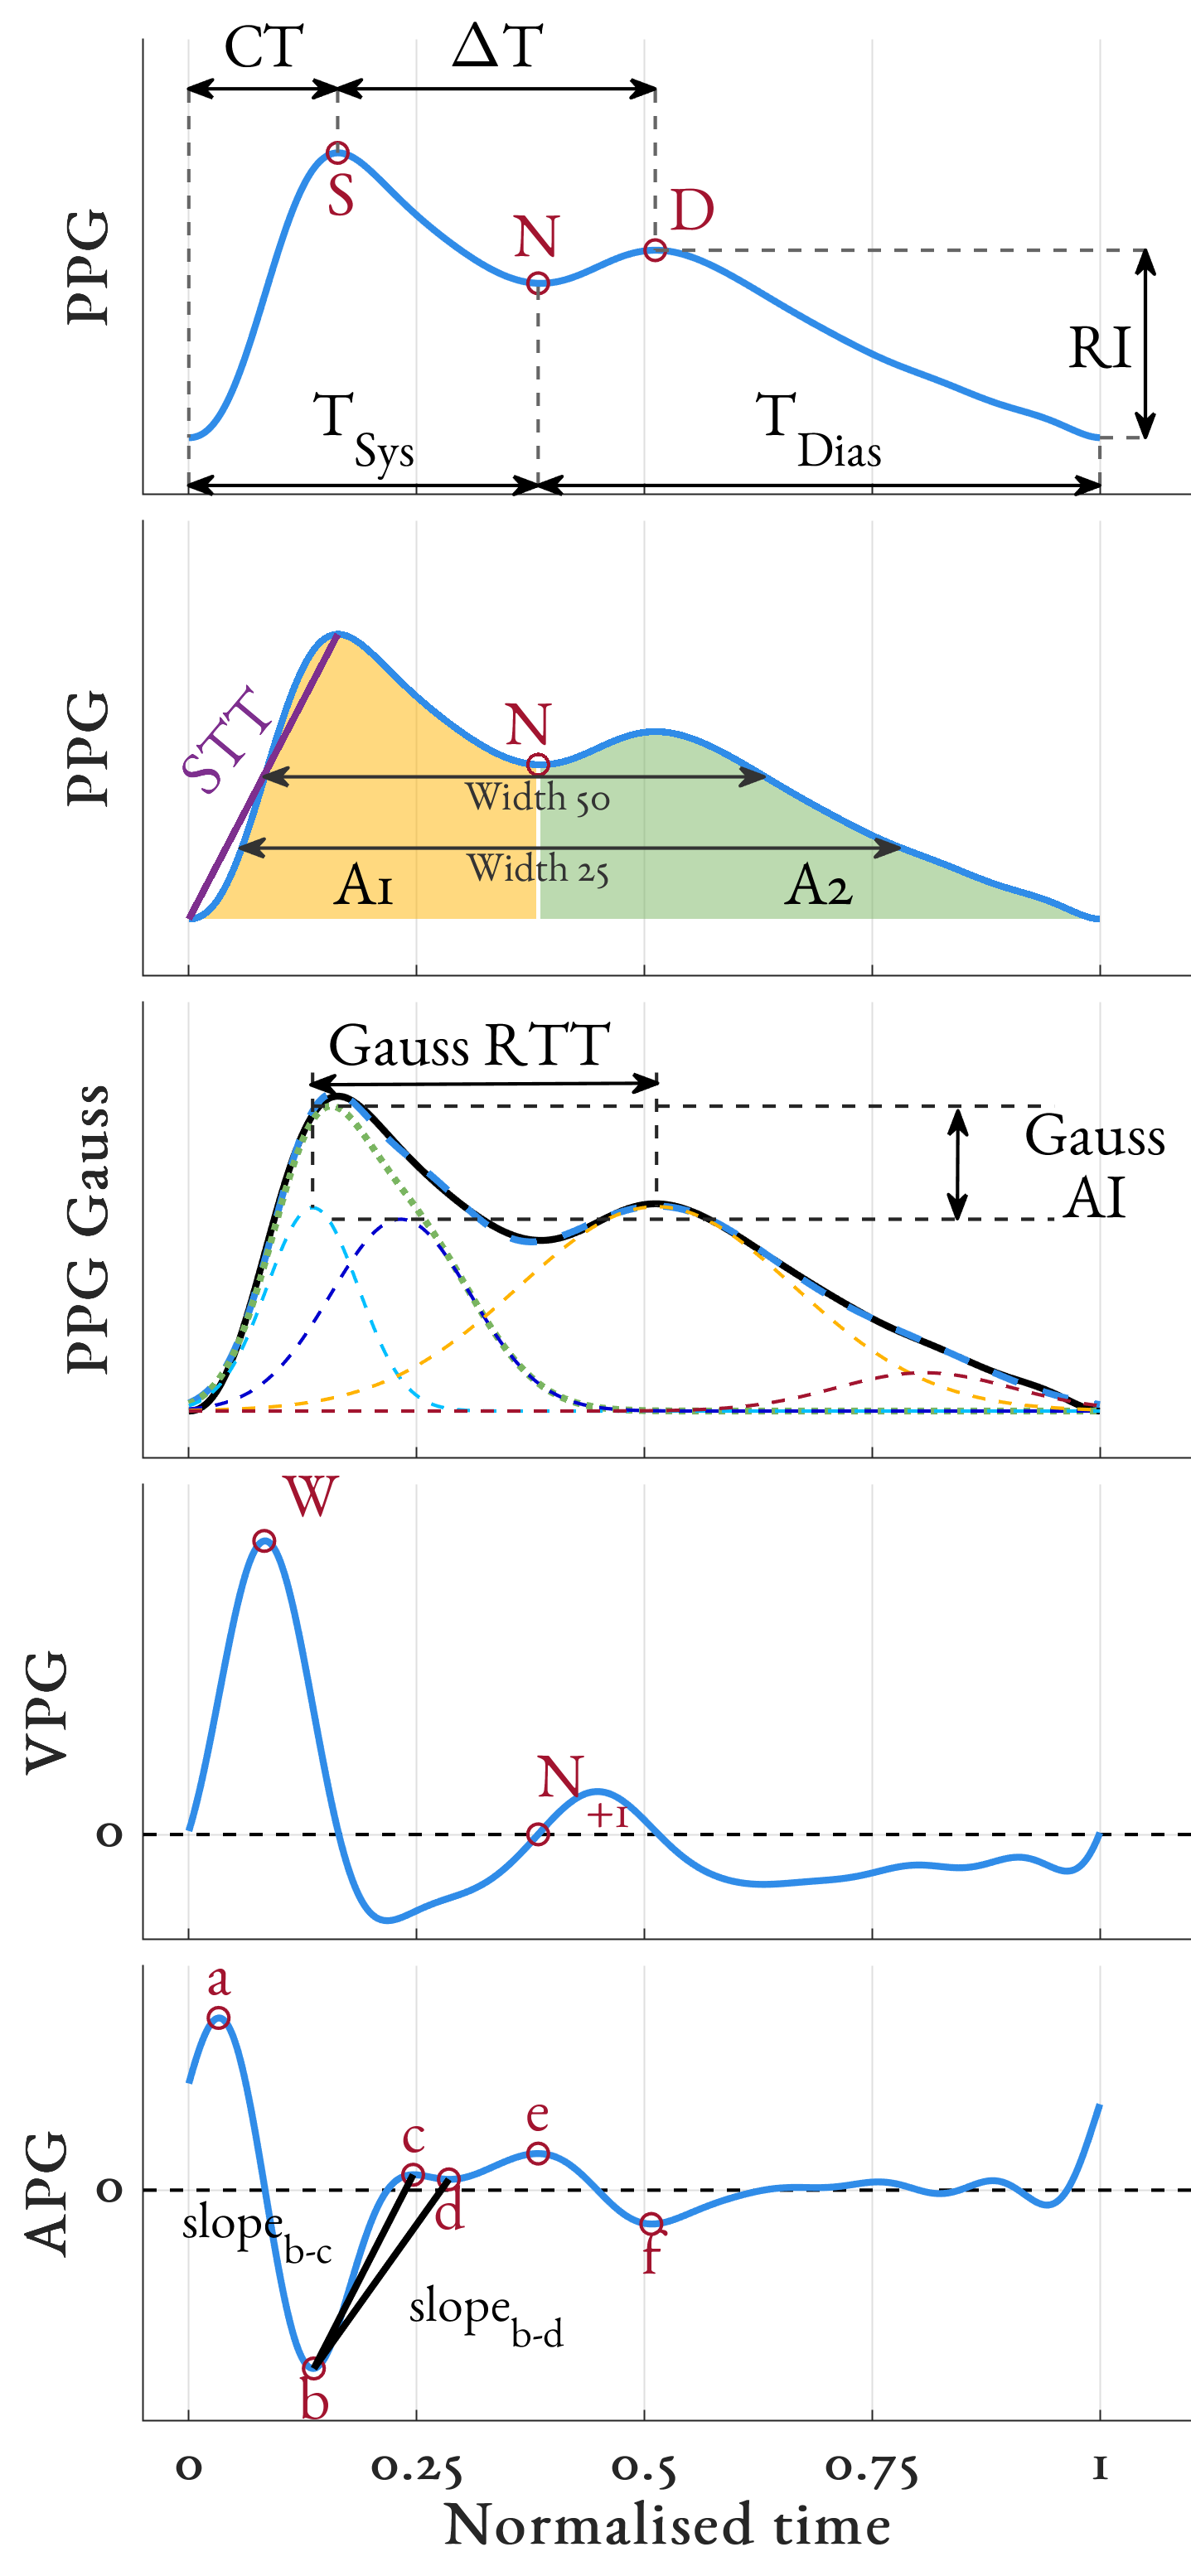
\includegraphics[height = \figHeight]{PPG_feats_rest.png}
		\caption{}
	\end{subfigure}
	~
	\begin{subfigure}{.24\textwidth}
		\centering
		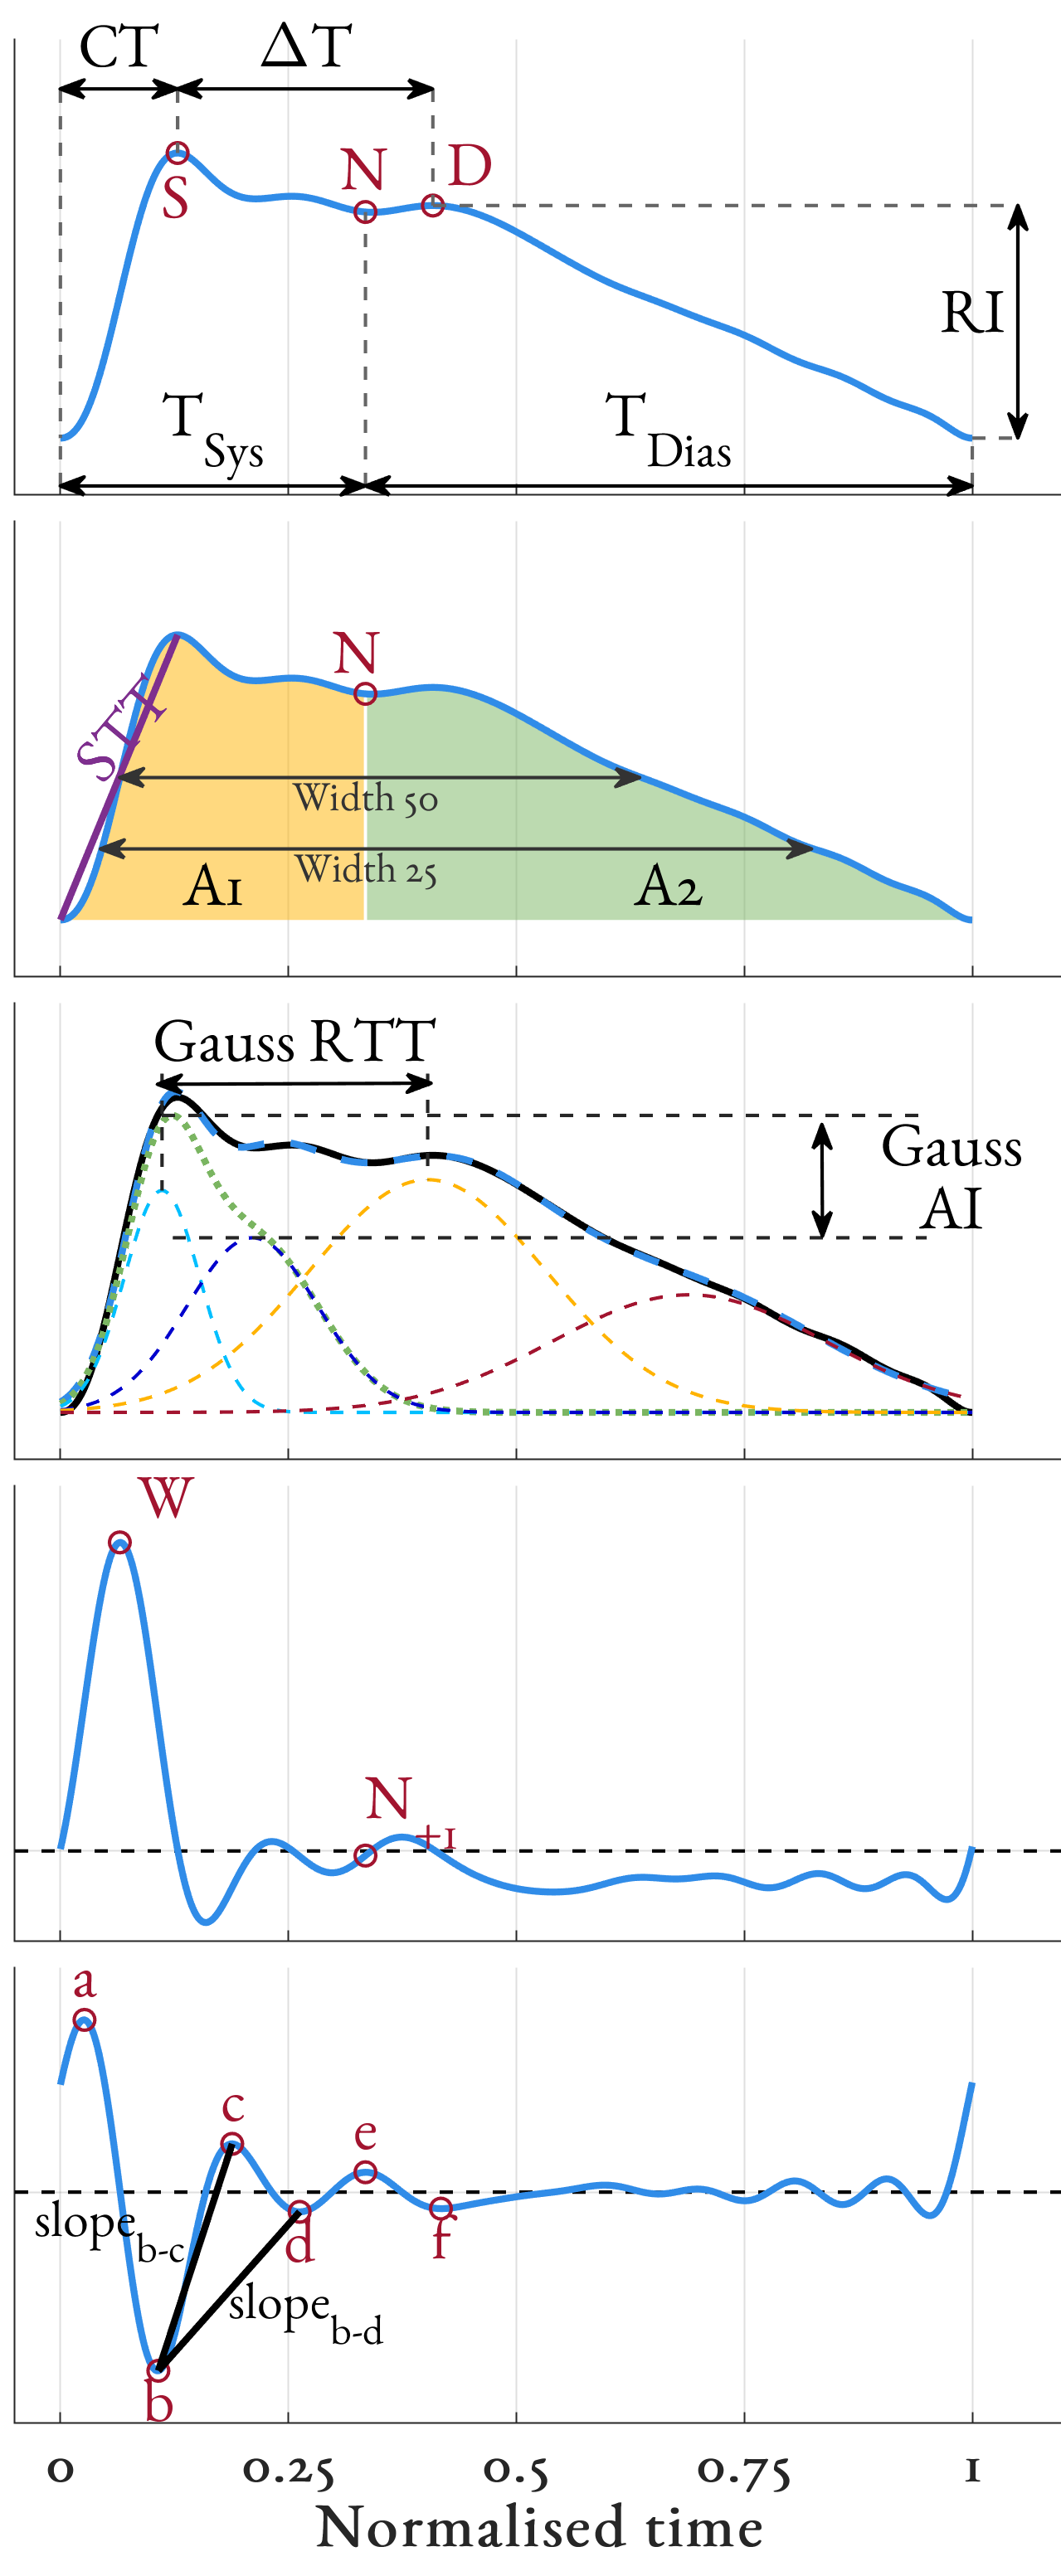
\includegraphics[height = \figHeight]{PPG_feats_dose_increase.png}
		\caption{}
	\end{subfigure}
	\begin{subfigure}{.24\textwidth}
		\centering
		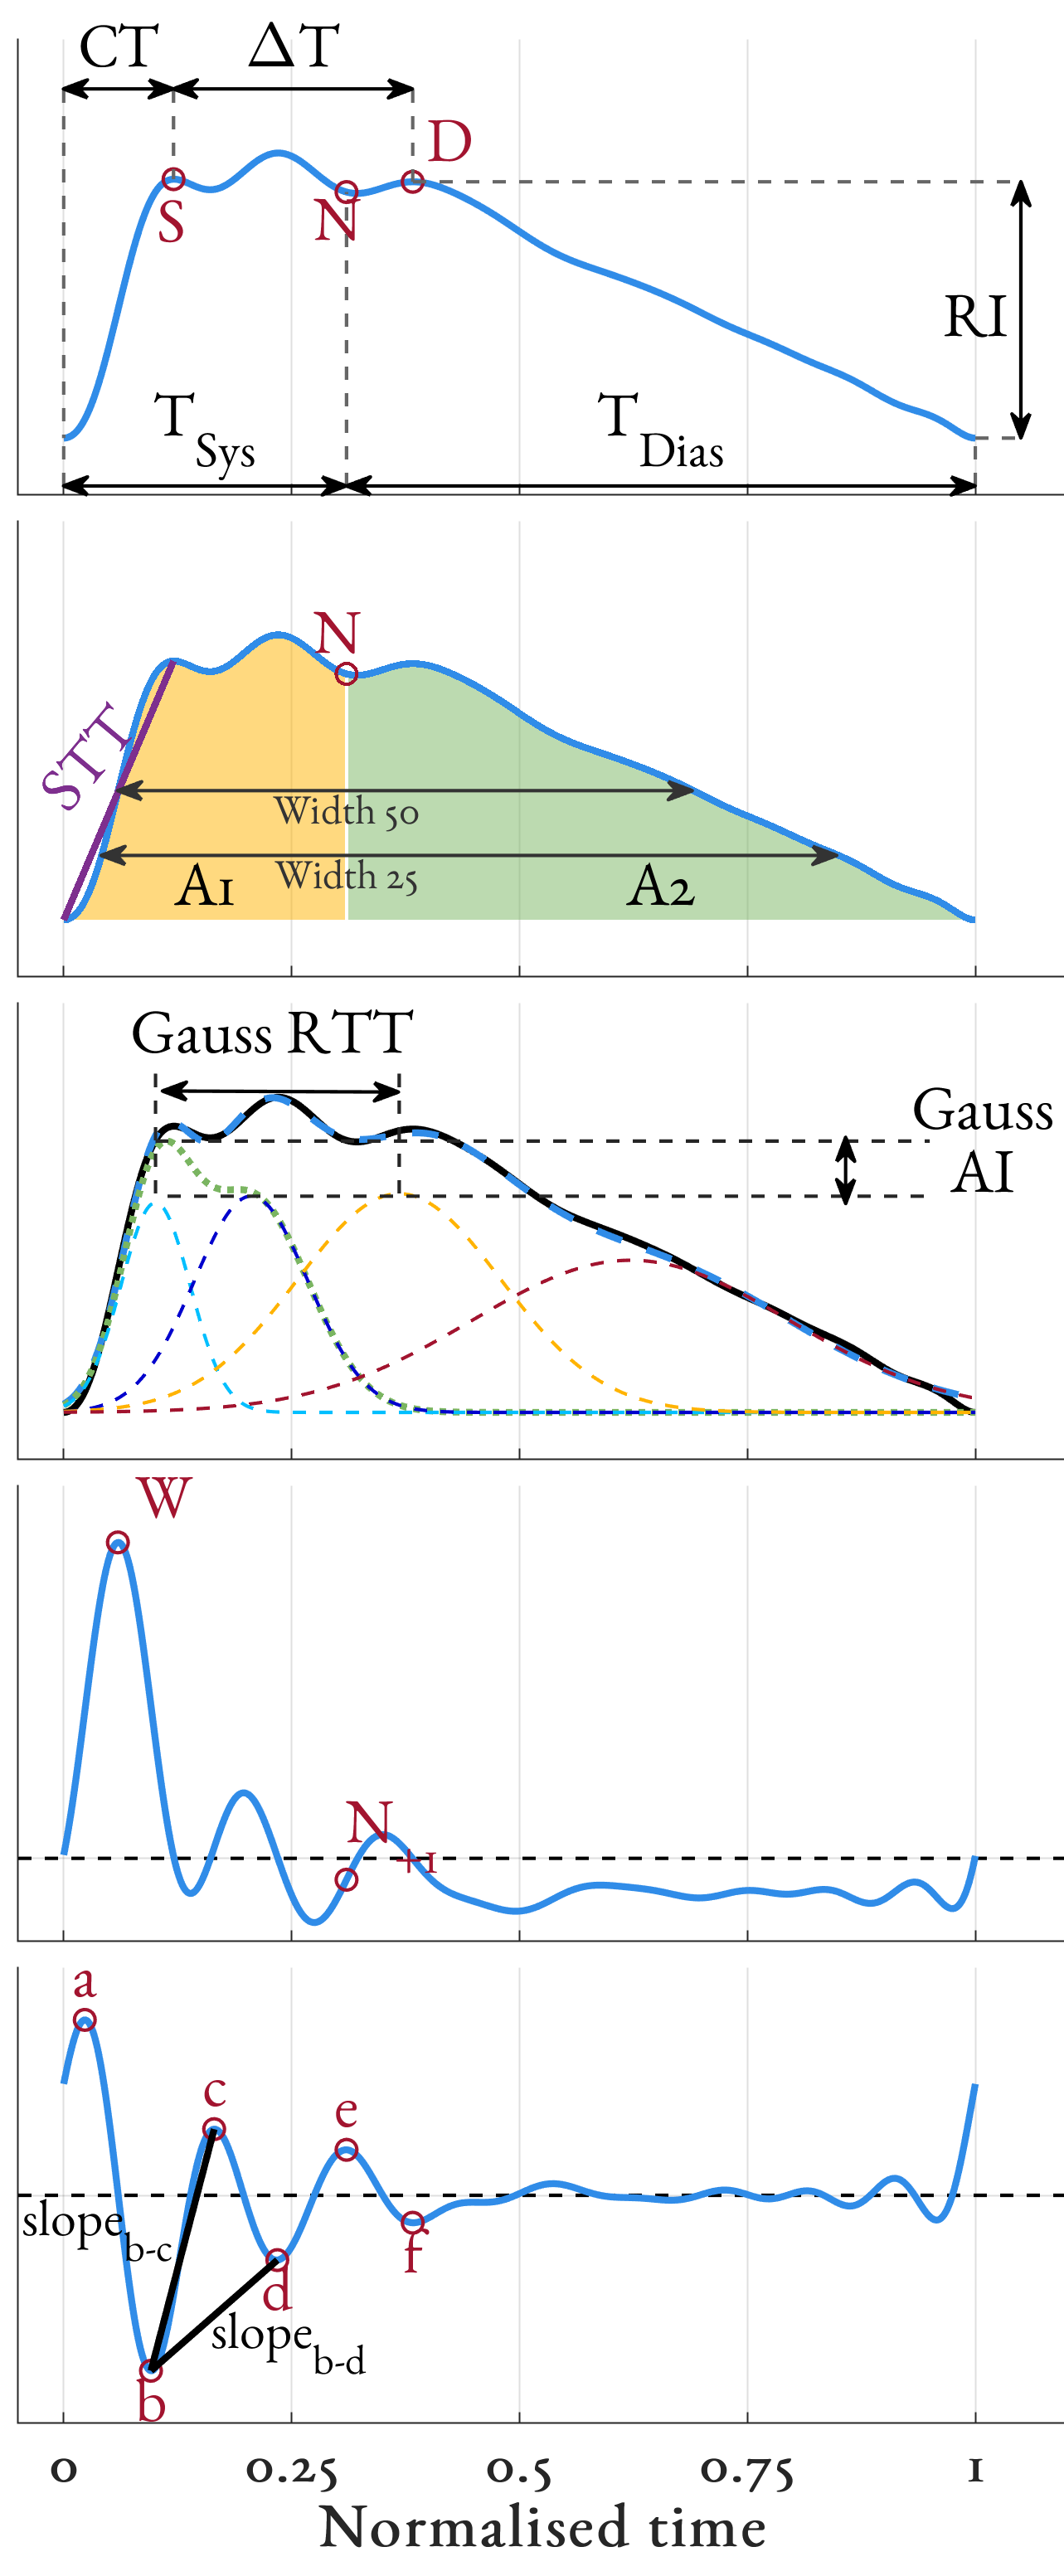
\includegraphics[height = \figHeight]{PPG_feats_max_infusion.png}
		\caption{}
	\end{subfigure}
	~
	\begin{subfigure}{.24\textwidth}
		\centering
		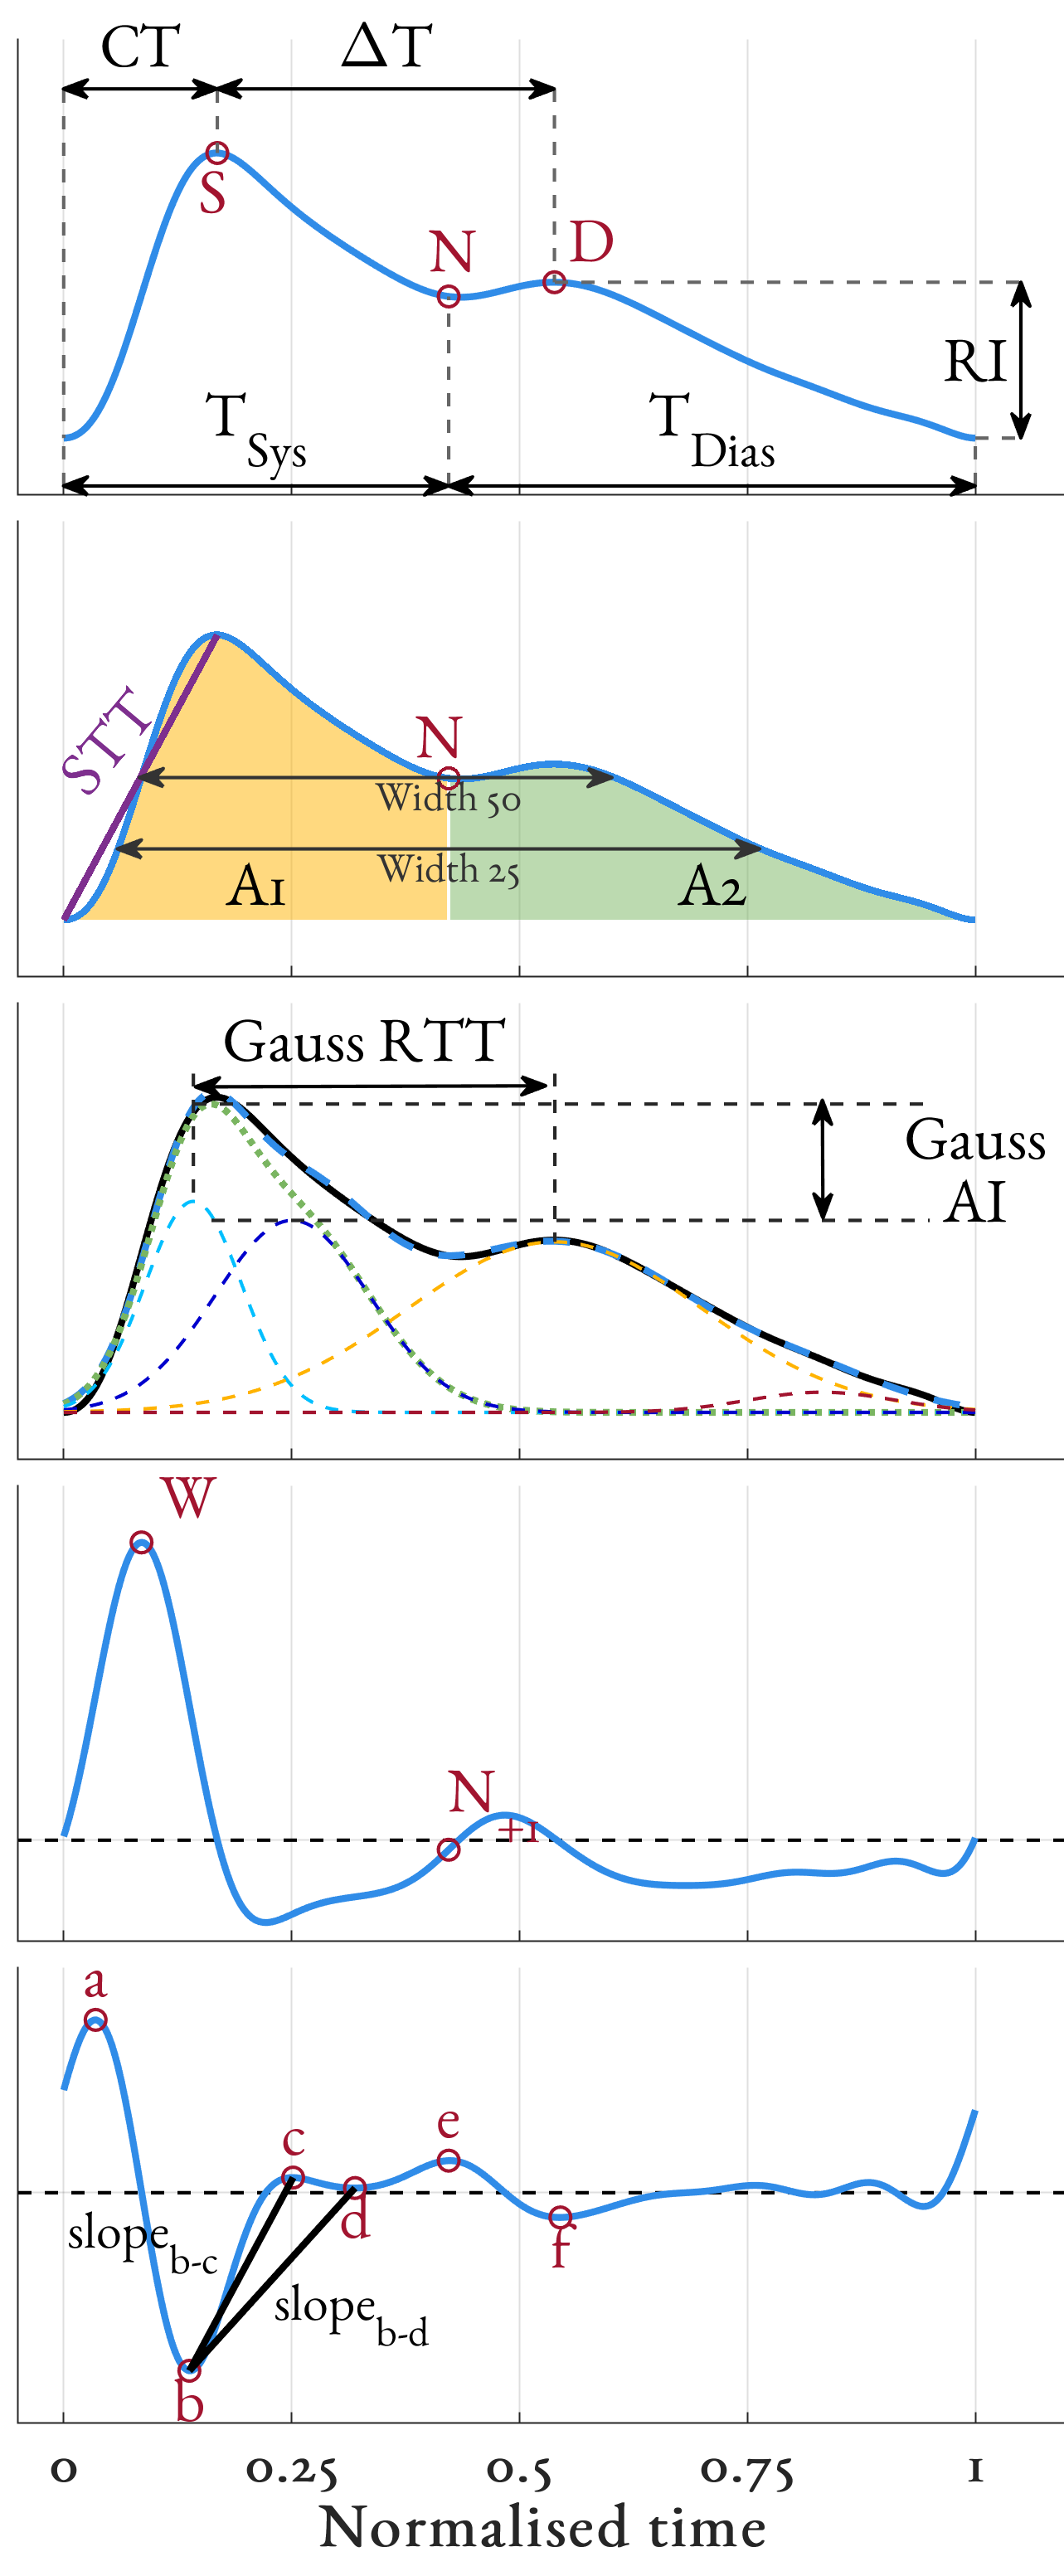
\includegraphics[height = \figHeight]{PPG_feats_washout.png}
		\caption{}
	\end{subfigure}
	\caption{Overview of the fiducial points detected and some of the features extracted from the PPG waveform for one individual (Male, Age: 24, BMI: 25.1) during the four stages of the study protocol: (a) rest, (b) dose increase, (c) maximum infusion, and (d) washout. Examples of the following features are provided: Crest time (CT), $\Delta$T, reflection index (RI), width\textsubscript{25}, width\textsubscript{50}, slope transit time (STT), A1, A2, Gaussian estimation of the transit time of the reflected wave (Gauss RTT) and augmentation index (Gauss AI), slope\textsubscript{b-c} and slope\textsubscript{b-d}. Acronyms: S - Systolic peak, N - Dicrotic notch, D - Diastolic peak, a-e - waves of the APG.}
	\label{fig:PPG_features_overview}
\end{figure}




% 
\small{
\afterpage{
\begin{longtable}{p{0.1\textwidth} p{0.4\textwidth} p{0.45\textwidth}}
	\caption{Summary of features extracted from the PPG. }
	\label{tab:PPG_features}\\
	\multicolumn{3}{c}{}\\
	\endfirsthead
	\multicolumn{3}{c}{\tablename\ \thetable\ -- \textit{Continued from previous page}} \\
	\multicolumn{3}{c}{}\\
	\hline
	\endhead
	\hline \multicolumn{3}{r}{\textit{Continued on next page}} \\
	\endfoot
	\hline
	\endlastfoot
		\textbf{Category} & \textbf{Feature notation and publication} & \textbf{Description or formula} \\
			\hline
			\hline
			\multirow{2}{*}{\shortstack[l]{PPG \\ morphology}} & Notch amplitude (N$_{amp}$) & Amplitude of the dicrotic notch (see \cref{fig:PPG_features_overview})\\
			& Reflective index (RI) \cite{Padilla2006} & Amplitude of the diastolic peak (see \cref{fig:PPG_features_overview}) \\
			& $\Delta$ T \cite{Elgendi2012}& Time from systolic peak to diastolic peak (see \cref{fig:PPG_features_overview}) \\
			& Crest Time (CT) \cite{Millasseau2002} & Time from onset to systolic peak (see \cref{fig:PPG_features_overview})\\
			& T\textsubscript{Sys} \cite{Ahn2017} & Time in systolic phase (see \cref{fig:PPG_features_overview})\\
			& T\textsubscript{Dia} \cite{Ahn2017} & Time in diastolic phase (see \cref{fig:PPG_features_overview})\\
			& T\textsubscript{Ratio} \cite{Ahn2017} & T\textsubscript{Sys}/T\textsubscript{Dia}\\
			& Slope transit time (STT) \cite{Addison2016} & Slope of straight line from onset to peak (see \cref{fig:PPG_features_overview})\\
			& Stress-Induced Vascular Response Index (sVRI) \cite{Lyu2015} & $\mu$\textsubscript{Dias}/$\mu$\textsubscript{Sys}\\
			& A1 \cite{Wang2009a} & Area under PPG in systolic phase (see \cref{fig:PPG_features_overview})\\
			& A2 \cite{Wang2009a}& Area under PPG in diastolic phase (see \cref{fig:PPG_features_overview})\\
			& Inflection point area (IPA)\cite{Wang2009a} & A2/A1\\
			& Width$_{25}$ \cite{Elgendi2012} & Width of the PPG at 25 \% of its amplitude (see \cref{fig:PPG_features_overview})\\
			& Width$_{50}$ \cite{Elgendi2012} & Width of the PPG at 50 \% of its amplitude (see \cref{fig:PPG_features_overview})\\
			& Pressure index (PI) \cite{Shin2017} &  $\frac{t(N) - t(S)}{t(N) - t(W)} \times h$\\
			& Normalised Harmonic Area (NHA) \cite{Wang2009a} & $\sum_{n=2}^{N}FFT^2(f_n)/\sum_{n=1}^{N}FFT^2(f_n)$\\
			& Inflection and Harmonic area ratio (IHAR) \cite{Wang2009a} & (1-NHA)/ IPA\\
			& Skewness \cite{Slapnicar2019} & -- \\
			& Kurtosis \cite{Slapnicar2019} & -- \\
			\hline
			\multirow{2}{*}{\shortstack[l]{VPG \\ morphology}} & Sys\textsubscript{$\mu$} \cite{Sun2016} & Mean of VPG in the systolic phase\\
			& Sys\textsubscript{$\sigma$} \cite{Sun2016}& Variance of VPG in the systolic phase\\
			& Dia\textsubscript{$\mu$} \cite{Sun2016}& Mean of VPG in the diastolic phase\\
			& Dia\textsubscript{$\sigma$} \cite{Sun2016}& Variance of VPG in the diastolic phase\\
			\hline
			\multirow{2}{*}{\shortstack[l]{APG \\ morphology}} & $\frac{b}{a}$, $\frac{c}{a}$, $\frac{d}{a}$ \& $\frac{e}{a}$ \cite{Takazawa1998} &\\
			& Ageing index (AGI) \cite{Takazawa1998} & $\frac{b - c - d - e}{a}$\\
			& slope\textsubscript{b-c} \cite{Ahn2017} & Slope of a straight line between $b$ and $c$, normalised by $a$ (see \cref{fig:PPG_features_overview})\\
			& slope\textsubscript{b-d} \cite{Ahn2017} & Slope of a straight line between $b$ and $d$, normalised by $a$ (see \cref{fig:PPG_features_overview}) \\
			& PPG AI \cite{Pilt2014} & PPG augmentation index $d_{-2}/b_{-2}$ \\
			\hline
			\multirow{2}{*}{\multirow{2}{.12\textwidth}{Gaussian decomposition}} & A$_{g1-4}$, $\sigma_{g1-4}$, $\mu_{g1-4}$ & Amplitude, variance and mean of the four decomposed Gaussians \\
			& Gaussian augmentation index (Gauss AI) \cite{Radha2019} & $\max(g_s) - A_{g3}$ (see \cref{fig:PPG_features_overview}) \\
			& Gaussian reflection index (Gauss RI) \cite{Radha2019} & $\sum(g_s) - \sum(g_3)$ \\
			& Gaussian reflected wave transit time (Gauss RTT) \cite{Rubins2008} & $\mu_{g3} - \mu_{g1}$ (see \cref{fig:PPG_features_overview}) \\
			& Gaussian augmentation index\textsubscript{R} (Gauss AI\textsubscript{R}) \cite{Rubins2008} $^{\dagger}$ & $\frac{A_{g1} - A_{g2}}{A_{g1}}$ \\
			& Gaussian reflection index\textsubscript{R} (Gauss RI\textsubscript{R}) \cite{Rubins2008} $^{\dagger}$ & $A_{g3}/A_{g1}$ \\
			& Gaussian approximation of left ventricular ejection time (Gauss LVET) \cite{Couceiro2012} & See reference for definition \\
			& Gauss$_{Sys/Dias}$ * &$\sum(g_s)/\sum(g_d)$ \\
			& Gauss$_{A4/A1}$ * & $A_{g4}/A_{g1}$ \\
			& Gauss$_{\sigma4/A1}$ * & $\sigma_{g4}/A_{g1}$ \\
			\hline
			\multirow{1}{*}{PCA} & PPG PCA \textsubscript{1-3} \cite{Xing2020}  & First 3 principal components of PPG beat \\
			& VPG PCA \textsubscript{1-3} \cite{Xing2020}  & First 3 principal components of VPG beat\\
			& APG PCA \textsubscript{1-3} \cite{Xing2020}  & First 3 principal components of APG beat\\
			\hline
			\hline
			\caption*{\small{* Indicates features that, to the authors' knowledge, have not been previously implemented for \ac{bp} estimation. $^{\dagger}$ Note that there are two Gaussian indices referenced reflection index and augmentation index. We refer to the second set using the subscript R to reflect the authors: Rubins \textit{et al.}} $\mu$\textsubscript{Sys} and $\mu$\textsubscript{Dias} represents the mean of the PPG during systole and diastole respectively. $h$ is the height of the participant. $t$ is the time since the pulse onset. FFT is the fast Fourier transform. $g_i$ refers to the $i$\textsuperscript{th} Gaussian; $g_s$ = $g_1$ + $g_2$ representing the systolic wave; $g_d$ = $g_3$ + $g_4$ representing the diastolic wave. $\sum(g_i)$ is the area under the $i$\textsuperscript{th} Gaussian. }
\end{longtable}
}
}

\subsubsection{Gaussian decomposition}

Each PPG pulse (of unit amplitude and duration) was decomposed into the summation of four Gaussians \cite{Rubins2008}. The first two Gaussians represent the systolic component of the pulse, the second two Gaussians represent the diastolic component. This approach has the advantage of providing a representation of the PPG pulse without a reliance on fiducial point detection. Additionally, it allows for the modelling of reflected wave interactions which are thought to have a Gaussian profile \cite{Sola2019}. For a PPG pulse $\zeta$ we computed the modelled pulse, $\zeta$\textsuperscript{Gauss}, as:

\begin{equation}
	\text{$\zeta$\textsuperscript{Gauss}}(t, \Theta) = \sum_{i=1}^4 g_i(t, \theta _i)
\end{equation}
where $g_i$ represents the $i$\textsuperscript{th} Gaussian component:
\begin{equation}
	g_i(t, \theta _i) = A_{gi} \times	e^{-\frac{(t-\mu_{gi})^2}{2\sigma_{gi}^2}}
\end{equation}
$t$ is the time duration for the PPG pulse, and $\theta _i$ is a vector, [$A_{gi}$, $\mu_{gi}$, $\sigma_{gi}$], containing the respective amplitude, mean and variance of each Gaussian. $\Theta$ = [$\theta _1$, $\theta _2$, $\theta _3$, $\theta _4$] and thus Gaussian decomposition parameterises each PPG beat into 12 components. To determine the optimum value for $\Theta$, $\hat{\Theta}$, we implemented a bounded Levenberg-Marquart optimisation algorithm to minimise the root mean squared error loss, $L$\textsuperscript{Gauss}, between $\zeta$ and $\zeta$\textsuperscript{Gauss} given as:



\begin{equation}
\mathit{L^{\text{Gauss}}}(\Theta) = \sqrt{\frac{1}{N}\sum(\zeta-\zeta^{\text{Gauss}}(t, \Theta))^2}
\quad, \qquad \hat{\Theta} = \argmin_{\Theta} (\mathit{L^{\text{Gauss}}}(\Theta))
\end{equation}

The optimisation was bounded such that all parameters were positive and the amplitudes were all less than 1. $L$\textsuperscript{Gauss} is non-convex and therefore the optimised values were dependent on initial conditions. For the first beat, the initial conditions were: $\theta_1 = [1/2, 0.2, 0.01]$, $\theta_2 = [1/3 , 0.4,  0.01]$, $\theta_3 = [1/4, 0.6,  0.01]$, and $\theta_4 = [1/6, 0.8,  0.01]$. To encourage continuity of parameters from beat-to-beat, we used the optimised parameters for the previous beat as initial seeds for the optimisation of the current beat. Following the work of \cite{Wang2013}, we set the SQI\textsubscript{PPG} of each beat to 0 if the value of $\mathit{L^{\text{Gauss}}}(\hat{\Theta})$ for that beat was greater than 0.03.


\Cref{tab:PPG_features} provides a summary of the Gaussian decomposition features used. Together with the values of $\hat{\Theta}$, we implemented various features derived from the Gaussian decomposition that have been previously proposed as indicators of arterial stiffness in the literature\cite{Rubins2008,Couceiro2012}. Additionally, through observations of Gaussian decomposition in our dataset, we propose three new features: the ratio of the systolic component to the diastolic component (Gauss$_{Sys/Dias}$); the amplitude of the fourth Gaussian scaled by the amplitude of the first Gaussian (Gauss$_{A4/A1}$); and the variance of the fourth Gaussian scaled by the amplitude of the first Gaussian (Gauss$_{\sigma4/A1}$) (scaling by variance rather than amplitude of the first Gaussian gave a less informative parameter). \Cref{fig:PPG_features_overview} shows an example of Gaussian decomposition for a typical participant during the four main stages of the study protocol: rest, dose increase, maximum infusion, and washout. \Cref{fig:PPG_features_overview} also presents examples of feature extraction for Gaussian estimation of the transit time of the reflected wave (Gauss RTT) and augmentation index (Gauss AI).


\subsubsection{Principal components}

Principal component analysis (PCA) \cite{Abdi2010PrincipalAnalysis} maps high-dimensional data to a lower dimension along orthogonal principal components. These principal components account for the majority of the variation in the original data and therefore highlight regions of significant change in the PPG, VPG and APG signals. We computed PCA features using the following steps:
% In comparison to classical PCA, each sample is analogous to a feature value and each beat in the session represents a different observation of the feature set.

\begin{enumerate}
    \item Resample all good-quality beats (defined as an SQI\textsubscript{PPG} $> 0.8$) from the PPG, VPG and APG signals to be 100 samples in length using cubic spline interpolation.
    \item Pool all resampled PPG, VPG and APG beats from all participants to form 3 matrices: $\Psi$\textsubscript{PPG}, $\Psi$\textsubscript{VPG} and $\Psi$\textsubscript{APG} respectively. 
    \item Mean normalise each $\Psi$ matrix.
    \item Perform PCA on each $\Psi$ independently by computing the eigenvectors of the corresponding covariance matrix and extract the first 3 principal components that correspond to the largest eigenvalues.
\end{enumerate}

We extracted 3 principal components as this was found empirically to explain more than 85\% of the variation in the $\Psi$\textsubscript{PPG}, $\Psi$\textsubscript{VPG} and $\Psi$\textsubscript{APG} datasets. A visualisation of the computed PCA eigenvectors is provided in Supplementary Information SI: 1.


\subsection{Features from the ECG}

To preprocess the ECG waveform, we performed the following steps. To suppress the impact of baseline wander, the ECG was filtered using an 8$^{\text{th}}$-order Butterworth IIR high-pass filter with a cut-off frequency of 0.5 Hz. To suppress power-line interference, a 2\textsuperscript{nd}-order IIR notch filter with centre frequency at 50 Hz (the frequency of mains power in the UK) was used. We detected the QRS complex following the work of Pan and Tompkins \cite{Pan1985} and assessed the quality of the ECG (SQI\textsubscript{ECG}) following the work of Li \textit{et al.} \cite{Li2008}.

The features we extracted from the ECG are summarised in \cref{tab:ECG_features}. Features relating to complexity and entropy of the ECG have been previously proposed to track changes in BP \cite{Simjanoska2018, Yang2020}. These features quantify the level of regularity and unpredictability of fluctuations over a time series. Generally, a higher-level complexity indicates a more irregular dynamic system. A lower-level complexity indicates the presence of central trends or cyclical patterns. Changes in entropy of the ECG time series have been shown to track changes in heart rate variability (HRV) caused by myocardial ischaemia \cite{Leonarduzzi2010a} and also denote periods of cardiac arrhythmia \cite{Li2016}. We provide full details of the algorithms used in Supplementary Information SI: 2. 

\begin{table}[ht]
	\centering
	\caption{Summary of features extracted from the ECG.}
	\label{tab:ECG_features}
	\begin{tabular}{p{.3\textwidth} p{.65\textwidth}}
			\textbf{Feature notation and publication} & \textbf{Description or formula} \\
			\hline
			\hline
			Hjorth mobility \cite{Simjanoska2018} & Estimate of the signal's mean frequency (Equation SI 1)\\
			Hjorth complexity \cite{Simjanoska2018} & Estimate of the signal's bandwidth (Equation SI 2)\\
			Fractal dimension \cite{Simjanoska2018} & Computed using Higuchi's algorithm \cite{Higuchi1988} with $k_{max} = 17$\\
			Shannon entropy (SE) \cite{Simjanoska2018} & Uncertainty of information content based on probability distribution (Equation SI 3)\\
			Approximate entropy (approxEnt) * & Quantifies regularities of signal\\
			Sample entropy (sampEnt) * & approxEnt computed without self comparisons\\
			Multi-level sample entropy (MSE) * & Course approximations of sample entropy, computed at scales 2, 4, 6, 8 \\
			\hline
			\\
			\end{tabular}
			\caption*{* Indicates features that, to the authors' knowledge, have not been previously implemented for \ac{bp} estimation. Full details of the algorithms and equations used for computing each feature can be found in Supplementary Information SI: 2. }
\end{table}


\subsection{Pulse Arrival Time}
\ac{pat} has been shown previously to provide a beat-by-beat estimate of changes in arterial stiffness and therefore may be a good surrogate for BP \cite{Finnegan2021}. \ac{pat} and its corresponding SQI\textsubscript{PAT} was computed in the same manner as we have previously reported \cite{Finnegan2021}. We used \ac{pat} in a baseline model to compare the performance of PPG and ECG features for BP estimation. 

\subsection{Computing the reference BP values}
\label{sec:BP_ref}

Measurements of \ac{sbp}, \ac{map}, and \ac{dbp} using sphygmomanometer cuffs have known limitations depending on posture, cuff-inflation hypertension and cuff size \cite{Ogedegbe2010, Lakhal2018}. The sphygmomanometer cuff used in our study was programmed to inflate every minute. However, errors in cuff inflation prevented the Philips monitor from registering an accurate estimate, resulting in a missed data-point in the recorded BP time series. Therefore, data from the cuff was both noisy and sparse. In order to reduce the impact of these sources of error, we processed the cuff data using a cubic smoothing splines \cite{Pollock1993} algorithm. This allowed for both filtering and interpolation of the noisy blood pressure readings to a new sampling frequency f\textsubscript{BP} set as once per minute. Cubic smoothing spline defines a function, $\hat{f(t)}$, that minimises a loss $L^{\text{BP}}$:

\begin{equation}
L^{\text{BP}} = p \sum (y_i - \hat{f(t_i)})^2 + \int \hat{f''(t)}^2 dt
\label{eqn:splines}
\end{equation}
where $y_i$ are the observed BP values from the cuff, occurring at time $t_i$, $\hat{f''(t)}$ is the second derivative of $\hat{f(t)}$. $p$ is a constant that defines the relative weight placed on minimising the residual sum of squares against the 'roughness' (the accumulated second derivative) of the regressed signal $\hat{f}$. As all participants were studied under the same protocol, we implemented $p$ values for SBP, MAP and DBP ($p_{\text{SBP}}$, $p_{\text{MAP}}$ and $p_{\text{DBP}}$ respectively) that were common for all participants in the dataset. More details of the methods for computing the reference \ac{bp} values can be found in Supplementary Information SI: 3.
 
 
\subsection{Estimating changes in BP} 
\label{sec:model}

We processed PPG features and \ac{pat} similarly to the methods proposed in \cite{Finnegan2021}. This included: outlier detection to remove statistically significant deviations in values and a Kalman filter to reduce the effect of transient artefacts caused by noise. We then averaged the feature values within a window, $w$, of length 40s centred around each reference BP measurement (20s to the left, 20s to the right). Only beats of good quality, given by SQI\textsubscript{PPG} > 0.8 and SQI\textsubscript{PAT} > 0.8 respectively, were included in the window and if more than half of the window was deemed to be of bad quality, then the feature was not recorded for that window. We computed ECG features within the same window, $w$. If less than half of the window was deemed to be of good quality (SQI\textsubscript{ECG} > 0.8), then feature values were not recorded for that window. We handled missing data, caused by poor signal quality, by nearest neighbour imputation for each participant.


A schematic outlining our proposed steps for estimating $\Delta$BP is shown in \cref{fig:MOLLIE2_overview}. In this work, we adopted a \textit{hybrid calibration}\cite{Mukkamala2022a} approach in order to estimate $\Delta$BP using one of two ML regression models (LASSO+OLS or RF, defined in the sections below) as a function of an input feature set, $X$. We implemented four different feature sets based on the different signals being analysed in this study. For each of the following groups we restricted $X$ such that it includes features only from these sources: $X \in $ \{PPG, ECG, PPG+ECG, PAT\}. We refer to these models and feature set combinations as LASSO + OLS\textsubscript{PPG} for a LASSO + OLS model with a PPG feature set, RF\textsubscript{PPG + ECG} for a RF model with PPG + ECG feature set, and so on. 

We calibrated all feature and BP values to the individual participant using data recorded during the rest period of the study (first 5 minutes of the recording). We then removed all collinear features and implemented data augmentation to increase the size of the training set, $X$\textsubscript{Aug}. We used nested leave-one-subject-out cross-validation (LOSOCV) to train, tune and evaluate the models. For each fold of the LOSOCV, one participant in turn was set as the test participant. Data from $X$\textsubscript{Aug} set for all participants apart from the test participant were used to train and tune the models. Nested LOSOCV was used for model validation to optimise model hyperparameters ($\lambda$ for OLS+LASSO and $mtry$ for RF) with the aim of minimising \ac{rmse}. Data from $X$ for the test participant was then used to evaluate the performance of the model. We used the following metrics to evaluate model performance: \ac{rho_p}, \ac{rmse}, and \ac{mae}. Differences in performance metrics across all folds from the models were evaluated for statistical significance by a two-tailed Wilcoxon signed-rank test. We adjusted the $p$-values for multiple comparisons using the Benjamini-Hochberg method \cite{Benjamini1995}. This technique aims to control the number of type I errors (incorrectly rejecting the null hypothesis) by inflating the lowest $p$ values (see \cite{Benjamini1995} for more details).

\begin{figure}
	\centering
	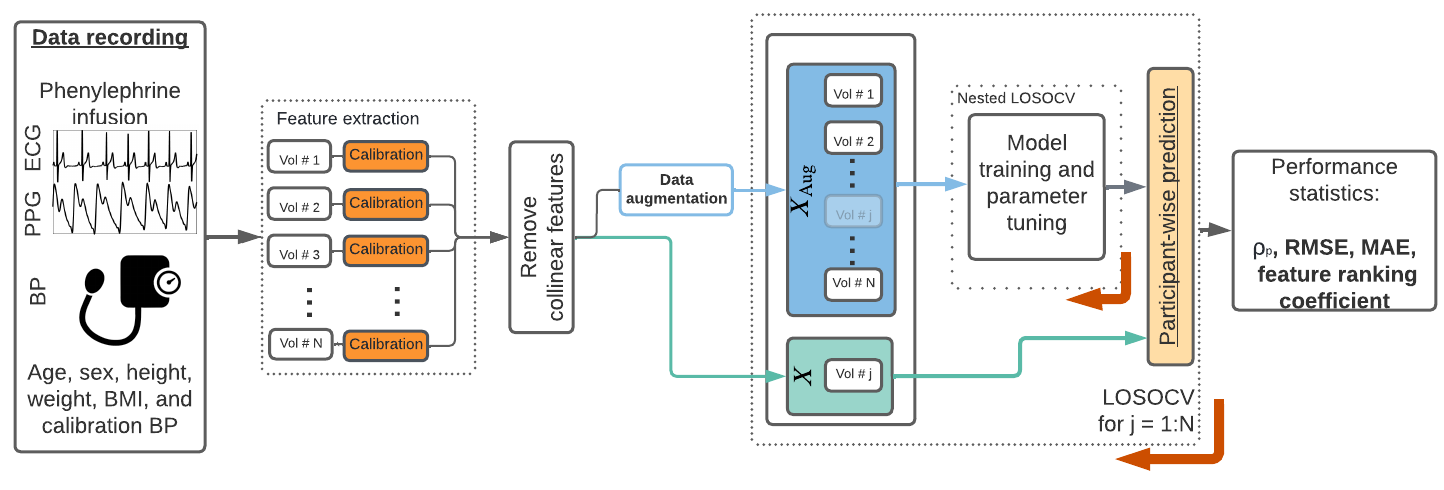
\includegraphics[width = \textwidth]{MOLLIE2flow.png}
	\caption{Schematic of the $\Delta$BP estimation pipeline for each of the proposed models. We extracted features from the PPG and ECG and averaged their values within a window of size 40s centred on times of cuff inflations. We then implemented a \textit{hybrid calibration} approach such that the proposed models estimate $\Delta$BP from a baseline calibration value determined during the rest period. Data augmentation was implemented to increase the training and validation set size by interpolating between cuff inflations. Models were trained and evaluated in a nested leave-one-subject-out cross-validation (LOSOCV) framework shown here by the iterator $j$ which indicates the test participant for that iteration. Participant $j$ was then removed from the training/ validation set ($X_{\text{Aug}}$) for that iteration.}
	\label{fig:MOLLIE2_overview}
\end{figure}




\subsubsection{Calibration}

We adopted a \textit{hybrid calibration} \cite{Mukkamala2022a} approach to personalise the estimation models for each participant in our dataset. In this work, we defined the baseline calibration value of BP (BP\textsuperscript{calib}) and waveform features ($f\textsuperscript{calib}$) as their respective mean values during the 5-minute resting period at the start of the study. In the specific example of one participant for whom no BP readings were taken during the rest period, we used the mean values in a one-minute window centred on the first cuff inflation as the calibration readings. For each participant, BP values were subtracted from their calibration value. Relative changes in feature values from their calibration values were used \cite{Natarajan2021}:

\begin{equation*}
    \Delta\text{BP} = \text{BP}  - \text{BP\textsuperscript{calib}}, \qquad \Delta f = \frac{f  - f\textsuperscript{calib}}{f\textsuperscript{calib}}
\end{equation*}
For all feature sets, $X$, we added participant age, sex, height, weight, \ac{bmi} and BP\textsuperscript{calib} as static categorical features. 

\subsubsection{Baseline reference}

For reference performance metrics, we implemented a simple baseline reference that assumed no BP changes for each participant from their baseline calibration value BP\textsuperscript{calib} (i.e. $\Delta$BP = 0). We refer to this as \textit{Baseline reference}.

\subsubsection{Removing collinear features}


Collinearity occurs when there is intercorrelation between multiple features \cite{Dormann2013, Kim2019}, thus violating the independent identically distributed (i.i.d.) assumption that is common in regression models. Additionally, the presence of collinearity inflates the variance of the regression parameters and makes it difficult to assess the importance of features. Collinearity in a feature set, $X$, can be highlighted by the condition number $\kappa$ representing the ratio of the largest singular value of $X$ to the smallest singular value. It can be computed as:

\begin{equation}
\kappa(X) = \left\|X^{+}\right\| \cdot \left\|X\right\|
\end{equation}
where $\left\|\cdot\right\|$ is the 2-norm of a matrix and $X^{+}$ is the pseudo inverse of the matrix $X$. Typically, a condition number greater than 30 is thought to indicate the presence of strong multi-collinearity in the dataset \cite{Kim2019}.

It is likely that collinearity exists in the feature sets presented in this paper as there are multiple features describing similar characteristics, for example entropies of the ECG or time durations of the PPG. In order to remove the effect of collinearity and to allow for parsimonious models, we removed collinear features by investigating the variance inflation factor (VIF) defined as:

\begin{equation}
    \text{VIF}_i = \frac{1}{1 - R_i^2}
\end{equation}

where $R_i^2$ is the unadjusted coefficient of determination for regressing the $i^{th}$ feature on the remaining ones. Removing collinear features is an iterative process where on each iteration, the feature with the largest corresponding $\text{VIF}_i$ is removed from the feature set until no features had a VIF greater than 10 (corresponding to $R_i = 0.9$)\cite{Kim2019}.




\subsubsection{Data augmentation}

We implemented data augmentation in order to increase the feature set size by incorporating information from feature values between the reference BP cuff inflations. As shown in \cref{fig:MOLLIE2_overview}, we performed model training and validation on the augmented feature set, hereafter referred to as $X$\textsubscript{Aug}, and performance metrics were reported using the original dataset $X$. We constructed $X$\textsubscript{Aug} by interpolating between the reference BP values for each participant using the cubic smoothing splines outlined above at a new frequency, $f$\textsubscript{BP} = 1/15 Hz (four measurements per minute, as opposed to once a minute) with a smaller window size, $w$ = 15s, to prevent overlapping windows violating the i.i.d assumption.


\subsubsection{Regression models}

The models we implemented to estimate $\Delta$BP are outlined below. Different models were built for estimating $\Delta$SBP, $\Delta$MAP and $\Delta$DBP.

\paragraph{LASSO + OLS}

To explore the linear relationship between each of the feature sets $X$ and $\Delta$BP, ordinary least squares (OLS) linear regression was implemented. In order to prevent over-fitting %, reduce the dimensionality%
and to improve model interpretability, we employed the Least Absolute Shrinkage and Selection Operator (LASSO) method to remove redundant features prior to linear regression. We refer to this model as LASSO+OLS. LASSO imposes the L1-norm penalty to the residual sum of squares using non-negative values of shrinkage parameter $\lambda$. LASSO allows removal of features by shrinking some feature coefficients, $\beta$, towards zero: 

\begin{equation}\label{eqn:LASSO}
\beta = \argmin_{\beta} (\sum_{i=1}^{N}(Y_i - X_i \beta)^2 + \lambda \sum_{j=1}^{M}|\beta_j|)
\end{equation}
where $Y$ is the target vector ($\Delta$BP values) of length $N$, and $M$ is the number of features. $|\beta_j|$ can therefore provide an indication of the relative importance of each feature. We optimised the $\lambda$ hyper-parameter by a nested LOSOCV loop. For each loop of the LOSOCV, LASSO feature selection was implemented and features with non-zero coefficients were used by OLS to compute $\Delta$BP estimates. 


\paragraph{Random forest}

To explore potentially non-linear relationships between $X$ and $\Delta$BP, we additionally built a Random Forest (RF) regression model. RF regression models utilise majority voting across multiple decision trees, each trained with a split criterion based on summed squared error (SSE) \cite{Genuer2008}. Each decision tree in a RF model was trained on a bootstrap of features. This approach reduces model variance whilst maintaining a low bias. As RF models select features upon training, we trained the model using all available features (i.e. without the need for LASSO). Typically, RF models are not very sensitive to choices in the number of trees ($N$\textsubscript{trees}), provided it is sufficiently high \cite{Genuer2008}. Therefore, we set the number of trees to 300. We optimised the number of features randomly selected for each node (labelled $mtry$) by a nested LOSOCV loop. The relative importance of each feature was assessed as the decrease in SSE averaged across all nodes and all trees that split based on that feature (see Genuer \textit{et al.} \cite{Genuer2008} for more details). 


\subsubsection{Feature ranking coefficient}

A key objective of this work was to highlight features that have strong predictive power for estimating $\Delta$BP. For each loop of the cross-validation (CV), features may have different relative feature importance values (provided by either LASSO or RF feature selection algorithms). To assess the variability of the relative importance, we computed a ranking coefficient. The ranks of all features were determined at each fold and normalised by the total number of features (1 being the highest rank, 0 being the lowest). For each feature, the distributions of the ranking coefficients across all folds were analysed.



% --------------------------------------------------------------------------- %
\section{Results}
% --------------------------------------------------------------------------- %
\subsection{Clinical study}


Thirty volunteers were recruited for our clinical study. We discarded the data from four participants from the analysis. For three of these participants, the reference ECG waveform did not include any periods of high-quality data as a result of errors in the connection of the ECG electrodes. For one participant there were errors recording the BP cuff data. Therefore, 26 participants made up our dataset. The demographics of the participants in the study whose data was used for analysis are shown in \cref{table:MOLLIE_demographics}. All participants were healthy with a median \ac{bmi} of 22.5 kg/m$^{2}$ and no history of cardiovascular disease. The median age of participants was 28 years and there was an even split of sexes (53.8\% female). On average, we achieved an increase of 20 mmHg in SBP, with a maximum increase of 40 mmHg in a subset of participants. 

\begin{table}[!hbt]
	\centering
	\caption{Demographics of the population in the clinical study. }
	\label{table:MOLLIE_demographics}
	\begin{tabular}{l | c}
	\hline
		\textbf{Descriptor} & \textbf{Value}  \\
		\hline
		Total number of participants & 26 \\
		\hspace*{0.5cm} Male & 12 \\
		\hspace*{0.5cm} Female & 14 \\
		Average length of session (mins)\textsuperscript{1} &  28.0 (0.1) \\
		Age (years)\textsuperscript{1} &  28 (9.0) \\
		Height (cm)\textsuperscript{1} &  170.0 (18.0) \\
		Weight (kg)\textsuperscript{1} &  69.5 (23.0) \\
		Body Mass Index (kg/m$^{2}$)\textsuperscript{1} &  22.5 (5.2) \\
		
		Reference maximum $\Delta$ BP per participant\textsuperscript{1} & \\
		\hspace*{0.5cm} $\Delta$ SBP (mmHg) & 20.0 (8.0)\\
		\hspace*{0.5cm} $\Delta$ MAP (mmHg) & 17.0 (10.0)\\
		\hspace*{0.5cm} $\Delta$ DBP (mmHg) & 15.5 (9.0)\\
		
		Reference $\Delta$ BP values\textsuperscript{2} & \\
		\hspace*{0.5cm} $\Delta$ SBP (mmHg) & 6.5 (10.4) \\
		\hspace*{0.5cm} $\Delta$ MAP (mmHg) & 5.3 (8.8)\\
		\hspace*{0.5cm} $\Delta$ DBP (mmHg) & 4.7 (8.2)\\
		
		
		\hline
	\end{tabular}
	\caption*{\textsuperscript{1} Participant-wise median (\ac{iqr}), \textsuperscript{2} mean (standard deviation) across dataset.}
\end{table}

\subsection{Removing collinear features}

\Cref{fig:collinear_features} (a) shows the correlation matrix of the total feature set (PPG + ECG + demographics), including 77 features. There were a large number of features (58.5\%) which were significantly correlations ($|\rho_p|$ >0.8, $p < 0.05$) with at least one other feature. This indicates a high level of collinearity, highlighted by a condition number $\kappa$ of 315. \Cref{fig:collinear_features} (b) shows the correlation matrix after removing all collinear features. The remaining dataset contained 45 features with a condition number $\kappa$ of 11, suggesting independence of features and encouraging parsimonious models. For completeness, Supplementary Information table SI 3 provides a list of the remaining features and the subset of the total feature set with which they have a strong correlation. Additionally, Supplementary Information table SI 3 provides the correlation with $\Delta$SBP for each feature across the whole cohort and on a participant-wise basis. 

\begin{figure}[ht]
	\centering
	\begin{subfigure}{.49\textwidth}
		\centering
		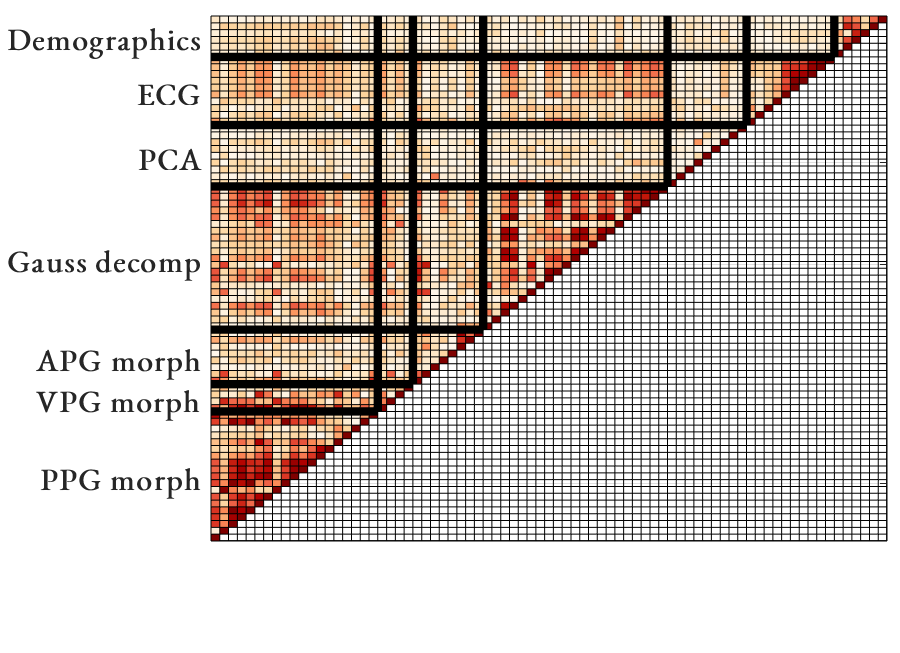
\includegraphics[height = 6cm]{before_collinear.png}
		\caption{}
	\end{subfigure}
	~
	\begin{subfigure}{.49\textwidth}
		\centering
		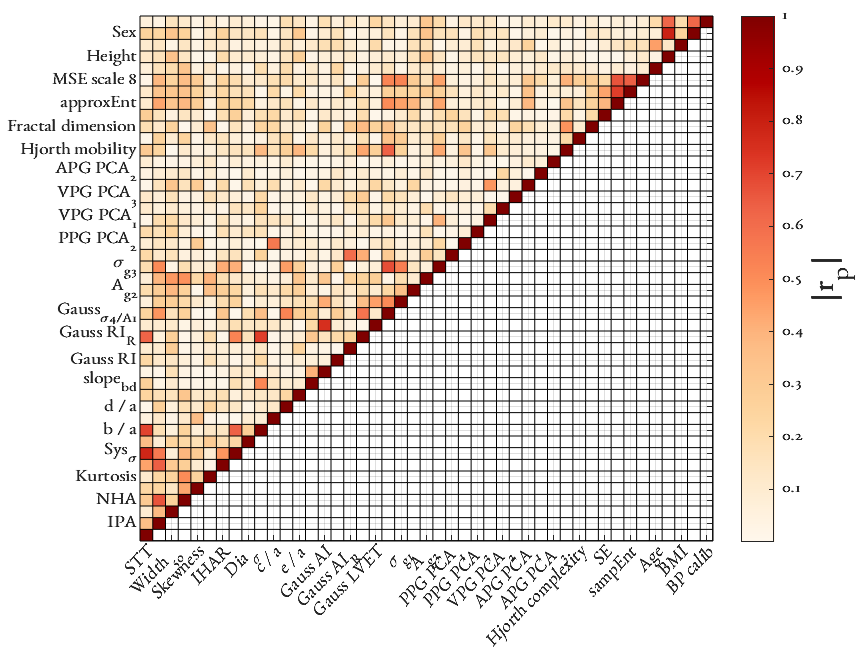
\includegraphics[height = 6cm]{after_collinear.png}
		\caption{}
	\end{subfigure}
	\caption{Results of removing collinear features in PPG + ECG feature set. Pairwise linear absolute Pearson's $|\rho_p|$ correlation matrix. (a) pre and (b) post removal of collinear features. Blank spaces represent non-significant ($p > 0.05$) or weak ($|\rho_p|$ < 0.2) correlations. For clarity of labelling on the post-collinear feature set (b), every other label is presented on the y-axis with the remaining labels on the x-axis. }
	\label{fig:collinear_features}
\end{figure}


\subsection{Comparing model performance}

\Cref{tab:final_results_SBP} shows the median and \ac{iqr} performance statistics for all models computed over all 26 folds of the LOSOCV for $\Delta$SBP. The results for $\Delta$MAP and $\Delta$DBP are provided in the Supplementary Information table SI 1 and table SI 2 respectively. We note large \ac{rmse} and \ac{mae} values for the \textit{baseline reference} indicating that participants experienced a significant change in their SBP values in response to the weight-based dosing of phenylephrine. 

All models outperformed results obtained with the \textit{baseline reference}, and all apart from LASSO + OLS\textsubscript{ECG} reported statistically significant $p$ values indicating that consistent improvements in performance statistics were observed ($p < 0.05$ for all). For the PPG, ECG and PPG+ECG feature sets, the RF model consistently achieved stronger performance metrics than LASSO + OLS. Statistically significant improvements were recorded only in \ac{rmse} and \ac{mae} ($p < 0.05$ for all). The Wilcoxon signed rank test failed to reject the null hypothesis of equal median $\rho_p$ between LASSO+OLS and RF. The PPG feature set significantly outperformed the ECG feature set for all performance metrics and regression models. The absolute difference in the median $\rho_p$, \ac{rmse}, and \ac{mae} between RF\textsubscript{PPG} and RF\textsubscript{ECG} was 0.19 ($p = 0.00007$), 1.04 mmHg ($p = 0.005$) and 0.53 mmHg ($p = 0.004$) respectively. RF\textsubscript{PPG} and RF\textsubscript{PPG + ECG} reported similar performance statistics with non-significant $p$ values, indicating that adding ECG features to a feature set of PPG features offers little or no performance gain. For PAT, LASSO + OLS significantly outperformed RF across all performance metrics ($p < 0.05$ for all). LASSO + OLS\textsubscript{PAT} achieved similar performance metrics to the RF\textsubscript{PPG + ECG}. LASSO + OLS\textsubscript{PAT} consistently resulted in the smallest \ac{iqr} for all performance metrics.

\Cref{fig:results} shows the (a) correlation and (b) Bland-Altman plots for $\Delta$SBP estimation using the RF\textsubscript{PPG + ECG} model. Individual participants are colour and marker-coded. The $\rho_p$ value of the overall estimation was 0.64. The median participant-wise correlation coefficient was 0.86 with a range of 0.34 to 0.95. \Cref{fig:results} (a) shows the histograms of the reference and estimated values. The reference $\Delta$SBP values ranged from -16.4 to 53.8 mmHg, but the estimated $\Delta$SBP values had a much tighter range of -3.37 to 22.2 mmHg. The bias of the overall error was 0.30 mmHg with a standard deviation of 8.05 mmHg (see \cref{fig:results} (b)). We note also an additional bias where large values of $\Delta$SBP were underestimated and small values were overestimated. At peak infusion, the median (IQR) value of $\Delta$SBP across the cohort was 20 (8) mmHg (see \cref{table:MOLLIE_demographics}). We found large errors in the data for the four participants whose $\Delta$SBP at peak infusion exceeded 30 mmHg.


Supplementary Information figures SI 3-4 shows the individual reference $\Delta$BP and estimated $\Delta$BP values using the RF\textsubscript{PPG + ECG} model across all participants in the study for SBP, MAP and DBP respectively.

\begin{table}[ht]
	\caption{Performance statistics of $\Delta$SBP estimation using the models proposed. Results are given as median (IQR) computed across all folds of the LOSOCV. Entries in bold indicate the best performance for that metric.}
	\label{tab:final_results_SBP}
	\centering
	\csvreader[
	tabular={l |c | c| c},
	table head= \textbf{Model name} & \textbf{$\rho_p$} & \textbf{\ac{rmse} \textsuperscript{*}} & \textbf{\ac{mae} \textsuperscript{*}}\\ \thickhline,
	late after line= \\,
	late after last line= \\  \hline,
    before line=\ifthenelse{\equal{\theFlag}{1}}{\vspace{-10pt} \\ \hline }{},
	head to column names,
	]
	{csv/SBP_results.csv} 
	{}
	{\modelName\textsubscript{\dataName} & \RMed \quad (\RIqr)  & \RmseMed	\quad (\RmseIqr) & \MaeMed \quad (\MaeIqr)}
	\caption*{\textsuperscript{*} results given in units of mmHg}
\end{table}



\begin{figure}[ht]
	\centering
	\begin{subfigure}{.49\textwidth}
		\centering
		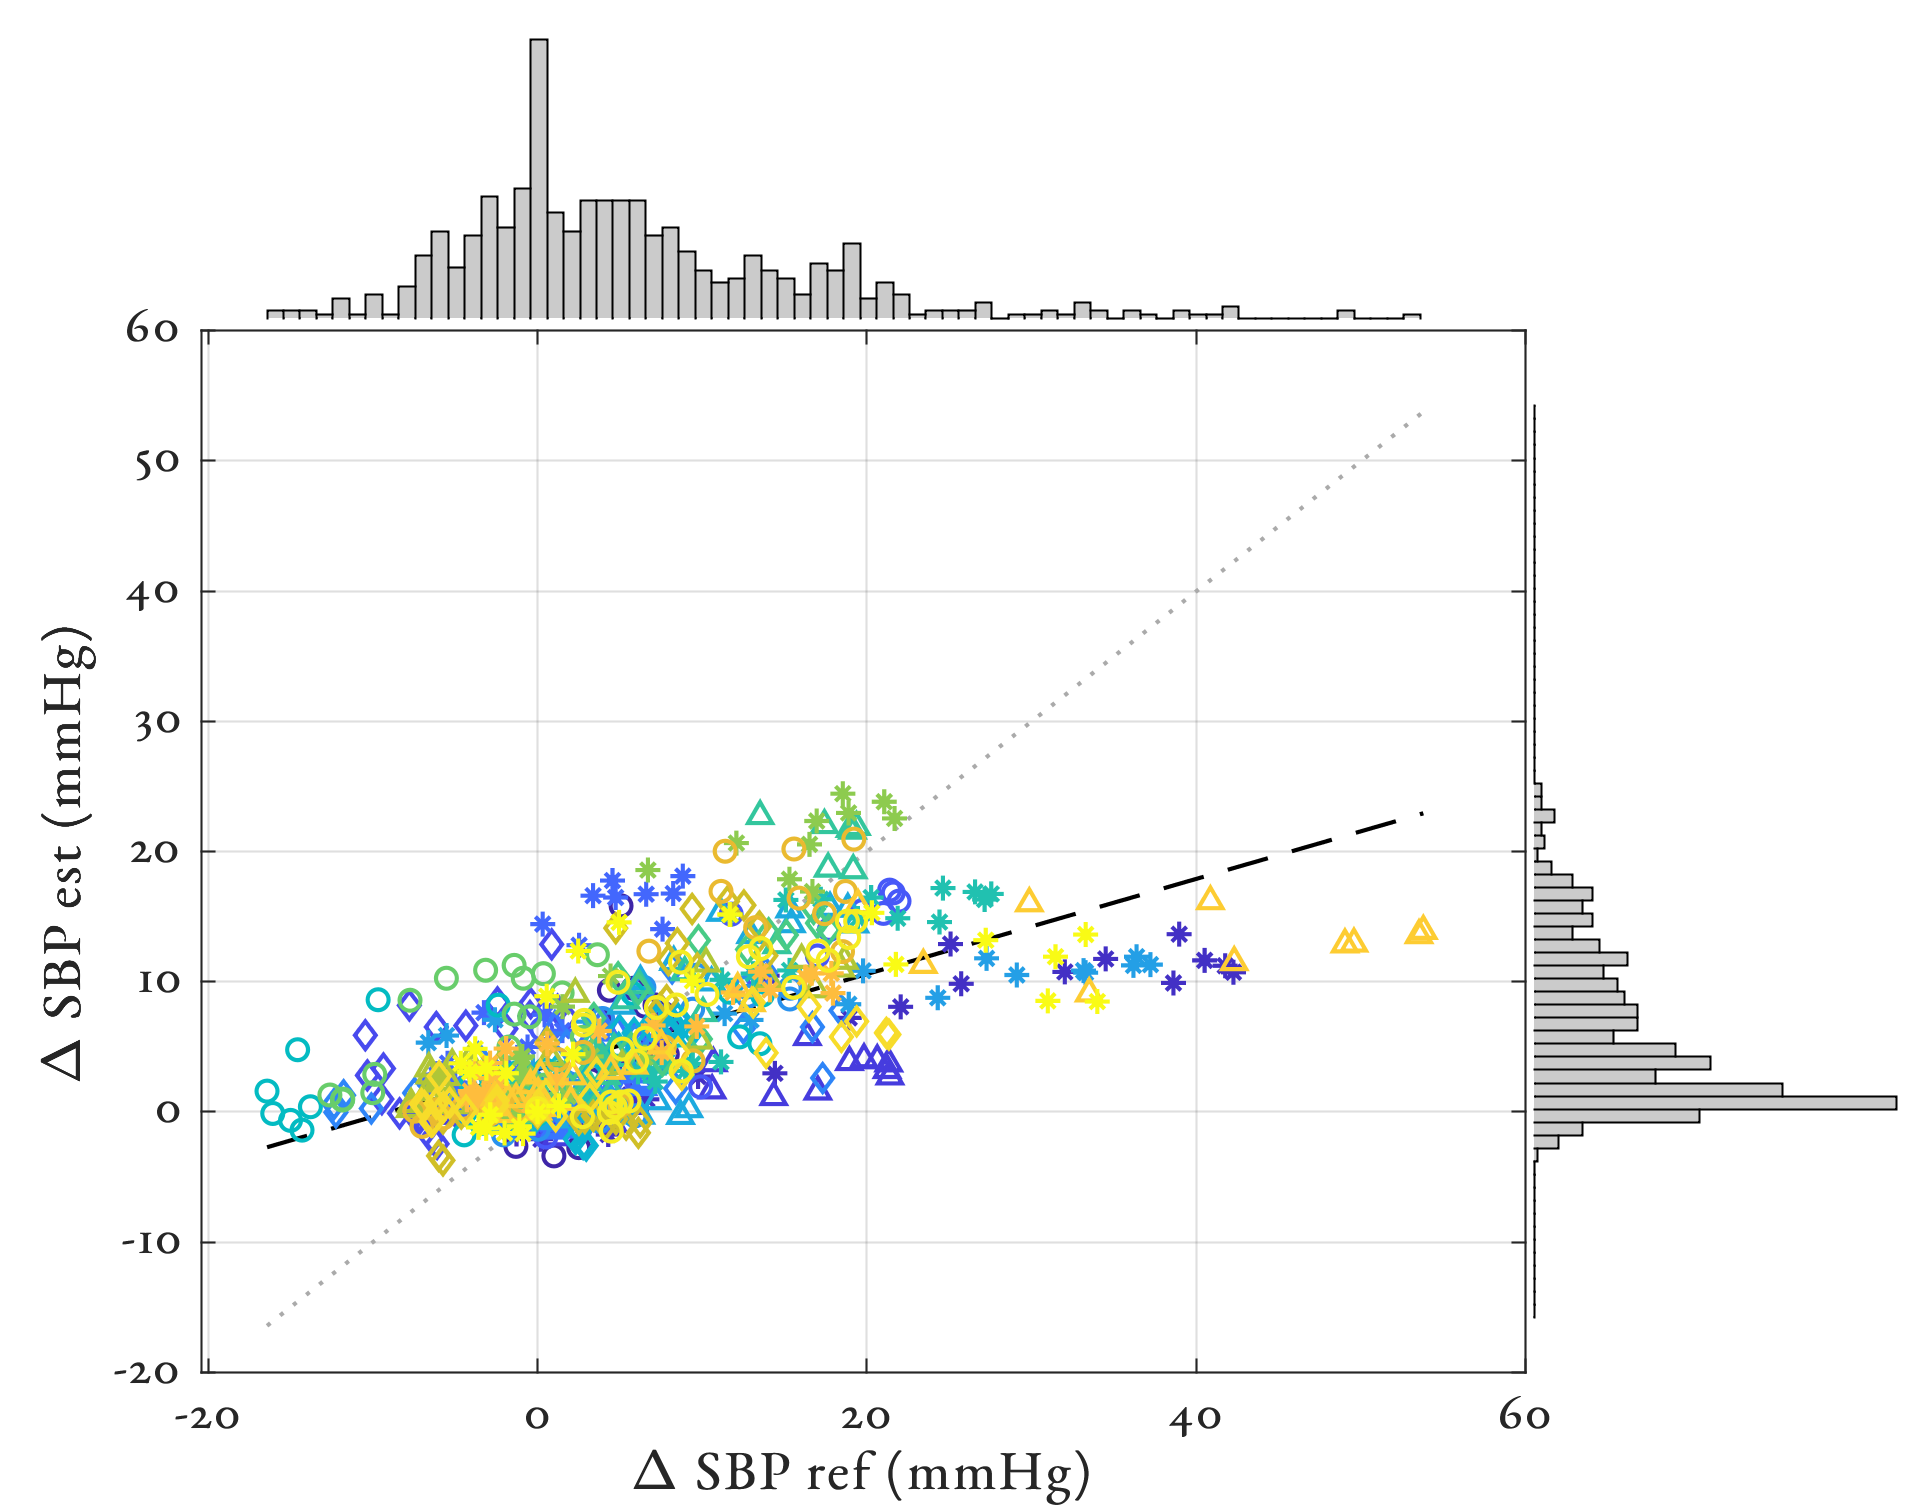
\includegraphics[width = \linewidth]{delta_BP_correlation.png}
		\caption{}
	\end{subfigure}
	~
	\begin{subfigure}{.49\textwidth}
		\centering
		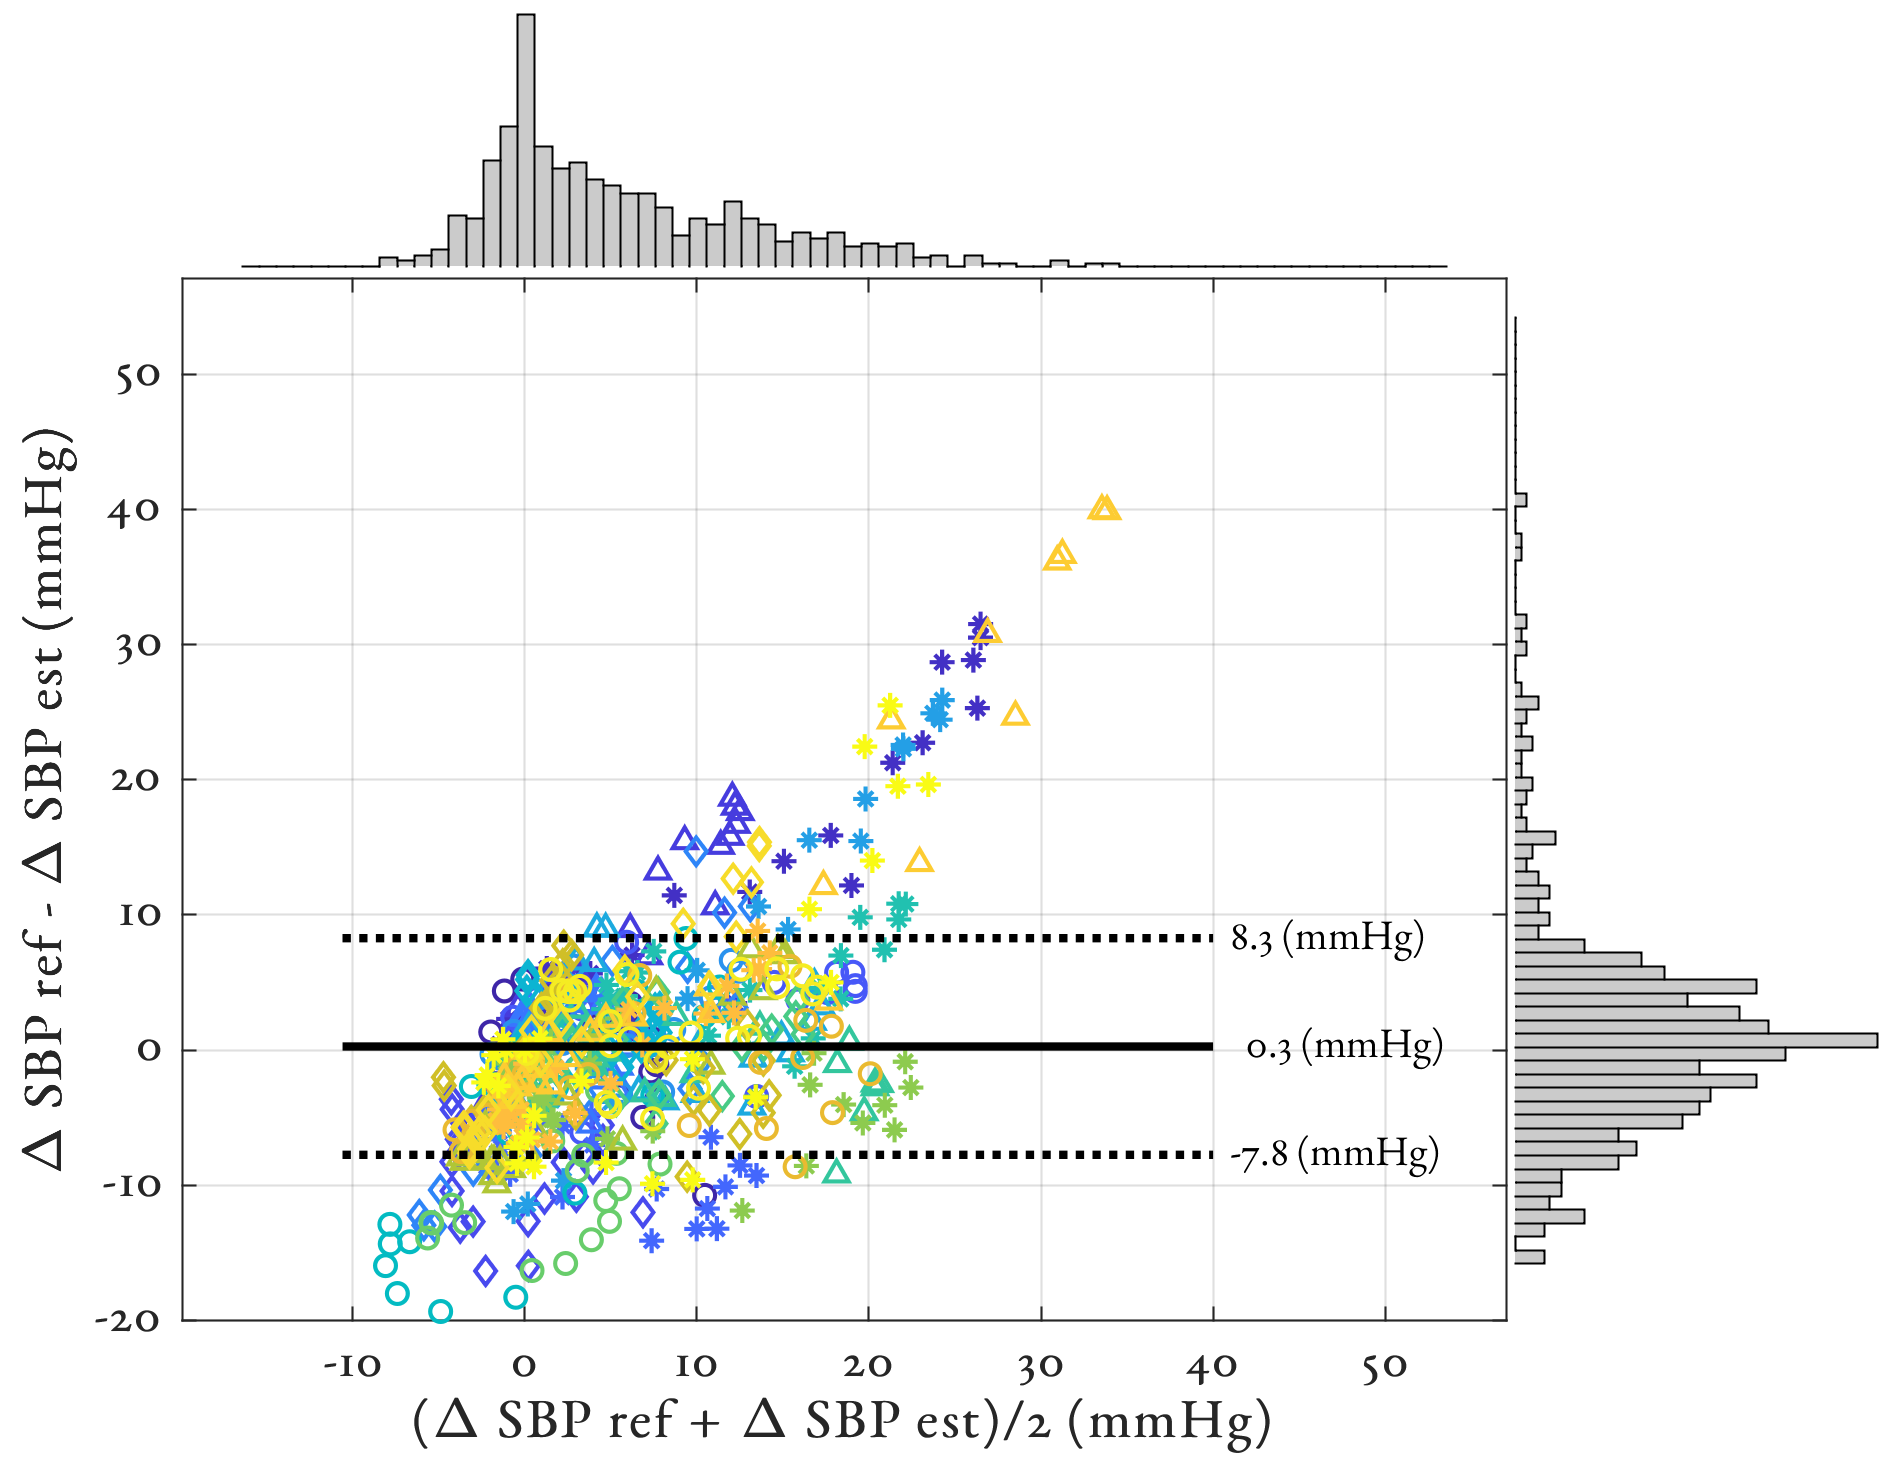
\includegraphics[width = \linewidth]{delta_BP_BA.png}
		\caption{}
	\end{subfigure}
	\caption{Agreement between the reference $\Delta$SBP values from the sphygmomanometer cuff and the estimated $\Delta$SBP using RF\textsubscript{PPG + ECG}. Individual participants are colour and marker-coded. (a) The correlation analysis, the overall correlation was 0.64, the median participant-wise correlation coefficient was 0.86 with a range of 0.34 to 0.95. Black striped line shows regression line. Grey dotted line shows line of unity. (b) The Bland-Altman analysis, the bias of the overall error was 0.3 mmHg with a standard deviation of 8.05 mmHg}
	\label{fig:results}
\end{figure}





\subsection{Feature importance}


\begin{figure}[ht]
	\centering
	\begin{subfigure}{.4\textwidth}
		\centering
		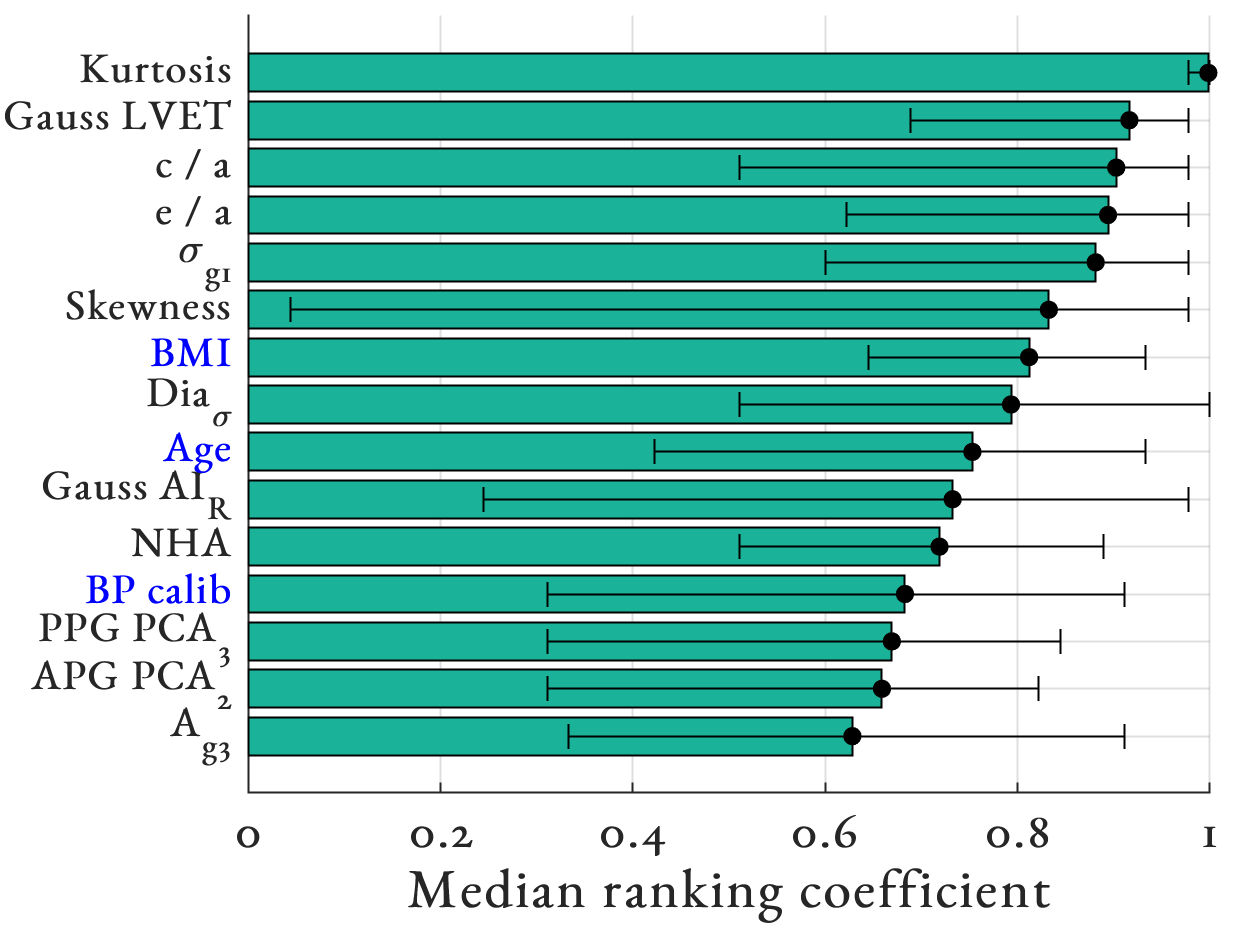
\includegraphics[height = 5cm]{feature_results_15_RF.png}
		\caption{}
	\end{subfigure}
	~
	\begin{subfigure}{.4\textwidth}
		\centering
		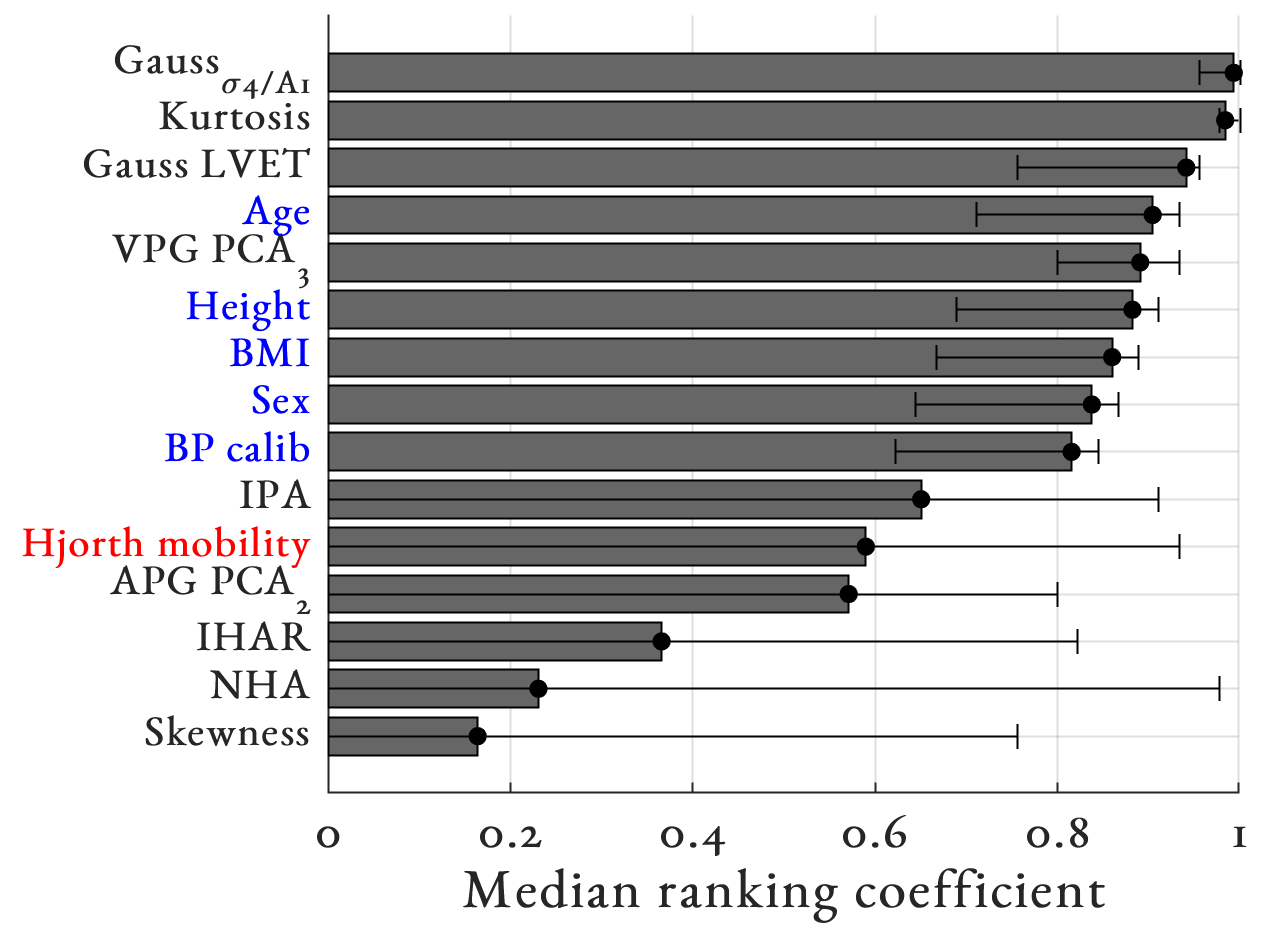
\includegraphics[height = 5cm]{feature_results_15_LR.png}
		\caption{}
	\end{subfigure}
	\caption{Median ranking coefficient for (a) random forest and (b) LASSO feature importance both with PPG + ECG feature set. Features are ordered by their respective median ranking coefficient. Error bars denote the range. Demographic features are highlighted in blue and ECG features in red for clarity. For brevity, only the top 15 features are provided here with the full list provided in Supplementary Information figure SI 2.}
	\label{fig:Ranking_coeffs}
\end{figure}

To mitigate the variations in the training data between folds of the LOSOCV, overall feature importance was assessed through using a ranking coefficient. \Cref{fig:Ranking_coeffs} shows the median (across folds) RF and LASSO ranking coefficients for the PPG+ECG feature set, with only the top 15 features shown (in \cref{fig:Ranking_coeffs}, all features are shown in Supplementary Information figure SI 2). The top five features as determined by the median RF ranking coefficient were: kurtosis, Gauss LVET, $e/a$, $c/a$, and \ac{bmi}. The top five features as determined by the median LASSO ranking coefficients were: Gauss$_{\sigma4/A1}$, kurtosis, Gauss LVET, age, VPG PCA\textsubscript{3}. Kurtosis had the highest feature importance in 22 out of 26 folds for RF and Gauss$_{\sigma4/A1}$ had the highest feature importance in 19 out of 26 folds for LASSO. In general, the ranking of features by LASSO followed the order of feature correlation values shown in Supplementary Information table SI 3. LASSO put a large emphasis on all demographic features, whereas RF put a comparatively low emphasis on height and sex. For RF, ECG features had very low importance with the strongest performing feature, sampEnt, having a median ranking coefficient of 0.35. LASSO placed slightly larger importance on ECG features, with Hjorth mobility having a median ranking coefficient of 0.60.

\Cref{fig:scatter_best_features} shows the relationship between $\Delta$SBP and the top 9 ranking, non-demographic, features from the RF\textsubscript{PPG + ECG} model. Different participants are coded by colour and marker to highlight clusters of features suggesting individual specific feature changes. Both Pearson's $\rho_p$ and Spearman's $\rho_s$ correlation coefficient are provided. Spearman's correlation indicates monotonic (but not necessarily linear) relationships and so may provide further insight into the RF models (see for example the scatter of $\sigma{g1}$).


\begin{figure}[ht]
	\centering
	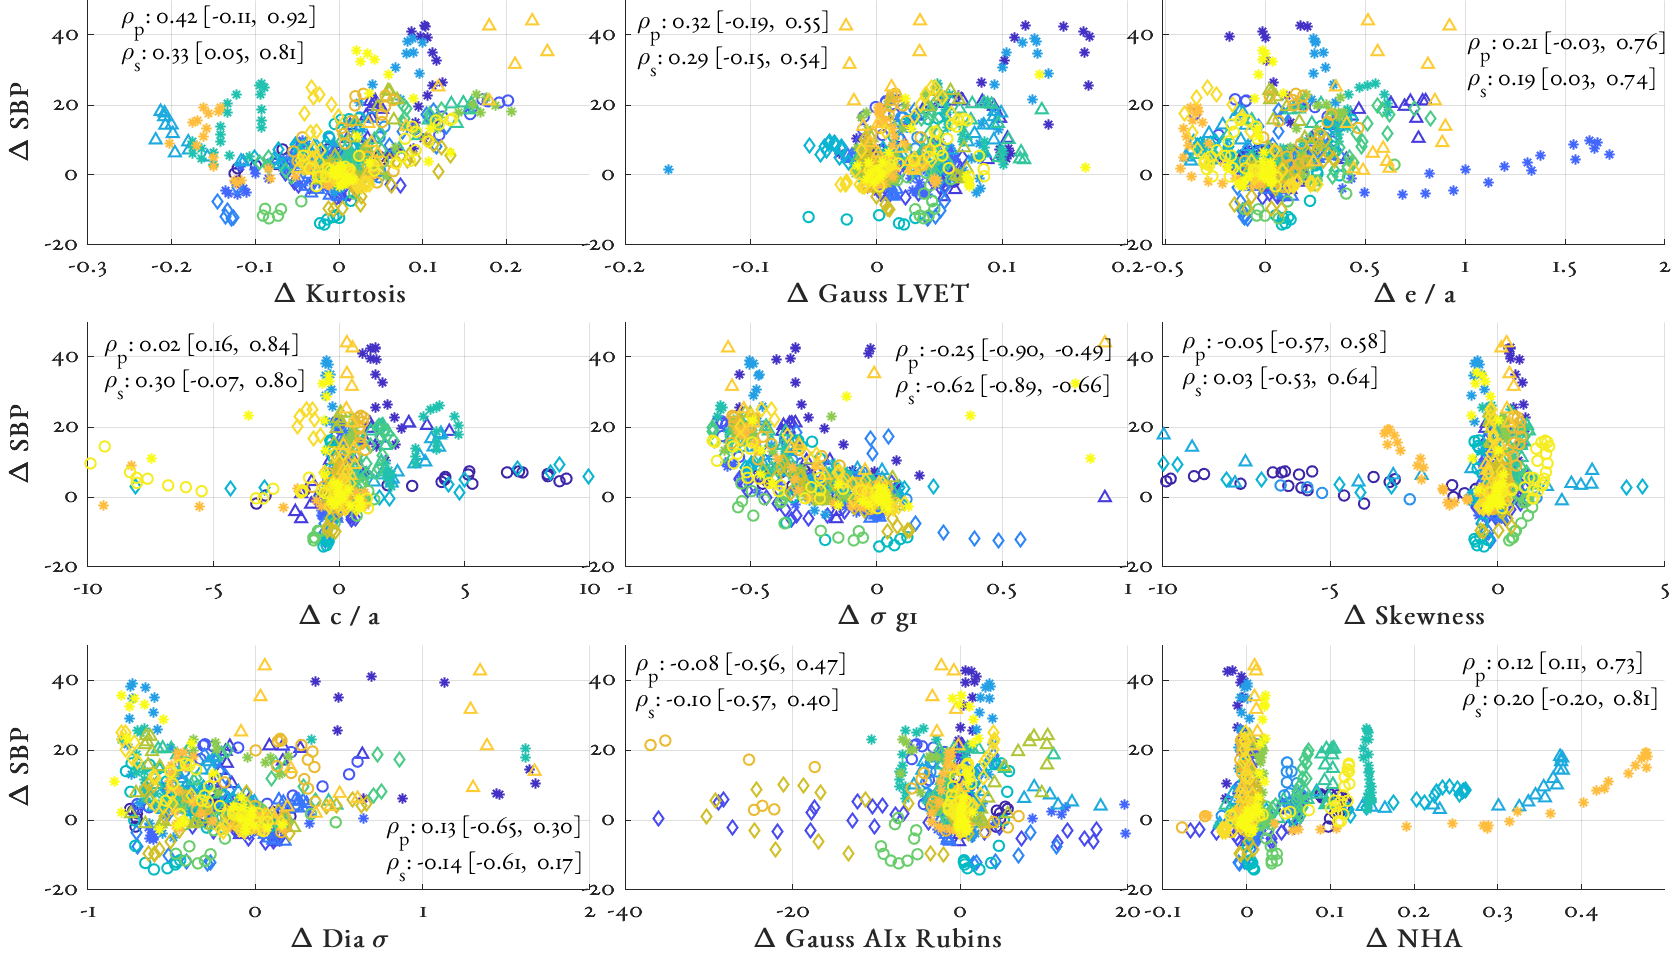
\includegraphics[width = \textwidth]{scatter_best_features.png}
	\caption{Relationship between top 9 ranking, non-demographic, features from the RF\textsubscript{PPG+ECG} model and $\Delta$SBP. Individual participants are colour and marker coded. Inter Pearson's $\rho_p$ and Spearman's $\rho_s$ correlation coefficient are shown as median and upper and lower quartiles. Additionally the 1st and 3rd quartiles of the participant-wise correlation coefficients are shown. Note that feature values have been both subtracted and divided by their value at baseline.}
	\label{fig:scatter_best_features}
\end{figure}

% --------------------------------------------------------------------------- %
\section{Discussion}
% -------------------------------------------------------------------------- %


This work describes the methods for the non-invasive estimation of $\Delta$BP in healthy participants using morphological features from the PPG and ECG waveforms. Changes in BP were induced by the infusion of phenylephrine using a weight-based dosing protocol, instead of being BP-target driven (although BP was constantly under review by the clinician to ensure safety of the participants). One of the key advantages of this study was that, in a relatively short period of time, and while remaining supine and still, the participants experienced a wide range of BP values. This helped to validate algorithms for non-invasive, cuffless, estimation of BP over a clinically useful range of $\Delta$SBP (-10 to 30 mmHg). 

% Among our participants, we observed heart rate values of around 40 beats per minute at peak infusion using this regimen. These decisions are outlined in the study protocol \cite{Harford2020} and we have further discussed the study in a previous publication \cite{Finnegan2021}. 

% We investigated the utility of features from the ECG and the PPG for tracking $\Delta$BP in the participants. 
The PPG and the ECG waveforms offer great potential for non-invasive monitoring due to their ubiquity and ease of acquisition. The PPG in particular can be acquired using wearable devices such as smartwatches or using video plethysmography \cite{Elgendi2019}. BP estimation using the PPG has been studied in a number of papers \cite{Elgendi2019}, however the best features and models have remained unclear. A single-lead ECG may be recorded by three electrodes or via capacitive coupling \cite{Taji2013}. The relationship between changes in BP and the ECG is governed by mechano-electric coupling (MEC). However, this connection is considered less robust to that of the relationship between the PPG waveform and BP. As a result, estimating $\Delta$BP from the ECG waveform has been explored in less detail in the literature. 

\subsection{Observed changes in the PPG waveform morphology}
\Cref{fig:PPG_features_overview} shows the changes in PPG beat seen for a typical participant during the four main stages of our study (a) rest, (b) dose increase, (c) max infusion and (d) washout. This includes a loss of a clear dicrotic notch (which is produced by the closing of the aortic valve and therefore marks the end of systole and the beginning of diastole) and a rising middle peak (often referred to as a tidal wave \cite{VonWowern2015} and thought to be caused by reflected waves at the renal arteries \cite{Baruch2011}) that can overshadow the initial peak seen at rest. These changes have been reported previously \cite{Sun2016,Sola2019,Elgendi2012} and are thought to be due to increasing amplitude and speed of reflected waves due to arterial stiffening. Additionally, they have also been shown to occur for age related arterial stiffening \cite{VonWowern2015}. Note that in \cref{fig:PPG_features_overview} (c) at maximum infusion, the tidal wave has a peak greater than that of the original systolic peak (see \cref{fig:PPG_features_overview} (b)). As the systolic peak is almost universally defined as the maximum of the PPG beat \cite{Charlton2018}, this may lead to the tidal wave being incorrectly classified as the systolic peak. In which case, features such as CT, $\Delta$T, and STT, which rely on accurate systolic peak detection would be significantly affected. To account for this, we detected the systolic peak as the first turning point of the PPG pulse above its midpoint, as can be seen in \cref{fig:PPG_features_overview} (c). We found that this definition was acceptable for our short, single perturbation study with minimal motion artefacts. 



\subsection{Model performance}


Typically, machine learning algorithms require a large amount of data in order to make robust estimations. In this work, we were limited by the number of participants in the study (N=26) and by the number of data points per participant (typically once per minute for the 28 minutes of the recording per participant). In order to overcome these limitations, the models were trained, tuned and evaluated with a LOSOCV framework. Additionally, we implemented data augmentation to increase the number of data points in our training set by interpolating between the cuff measurements using cubic smoothing splines with an additional 3 augmented measurements every minute. Across all models, this data augmentation statistically significantly improved the performance statistics at the $p < 0.001$ level, computed using a Wilcoxon signed rank test. \Cref{fig:collinear_features} (a) splits all features into groups (PPG, VPG, APG, Gaussian decomposition, ECG and demographics) and shows strong intra-group correlations indicating multi-collinearity in the dataset. We reduced feature collinearity by removing features with a VIF $> 10$. This increased the confidence of the model parameters, allowed for appropriate examination of feature importance and encouraged parsimonious models.  

For the PPG, ECG, and PPG+ECG feature sets, there were statistically significant improvements in \ac{rmse} and \ac{mae} when using the RF model compared to LASSO+OLS model at the $p< 0.05$ level as computed by the corrected Wilcoxon signed rank test, whereas a non-significant difference was found in $\rho_p$. This indicates that LASSO+OLS was able to appropriately detect directional changes in $\Delta$SBP, although it was unable to determine the magnitudes of the changes. This points to a calibration issue whereby the LASSO+OLS model was unable to approximate the feature gradients for each participant. RF models may have been better at calibrating to $\Delta$BP as these models allow for interactions between features and demographics. RF and LASSO both put a large emphasis on demographics (see \cref{fig:Ranking_coeffs}); however, in linear models these static features can only influence intercepts and not gradients. For RF\textsubscript{PPG+ECG}, a large importance was placed on \ac{bmi}, age, and BP\textsuperscript{calib}, all of which have a reported strong relationship with arterial stiffness and calcification within the arterial wall \cite{Ahn2017, Laurent2006}. Demographics are known to influence the PPG contour; in particular, c/a has been previously explored as a marker for age-related arterial stiffening \cite{Elgendi2012}. Interestingly, the RF\textsubscript{PPG+ECG} model puts little to no emphasis on the sex of the participant (see Supplementary Information figure SI 2) despite there being evidence of a sex-related dependency on the PPG morphology \cite{Dehghanojamahalleh2019}. We would recommend in future studies that the interactions between participant demographics may be accounted for in a linear model by implementing a linear mixed-effects model with random effects for parameters such as age and \ac{bmi}. We were unable to explore this line of work here due to the limited number of participants and their relative homogeneity. 


Despite interactions with demographics, a significant calibration issue still persisted. \Cref{fig:results} shows the results of $\Delta$SBP estimation using the RF\textsubscript{PPG + ECG} model via correlation and Bland-Altman analysis. The RF\textsubscript{PPG + ECG} model estimated $\Delta$SBP values to be in a much tighter range than was given by the reference and there were large errors found particularly at the high values. The largest errors found in all models occurred in the four individuals with the largest $\Delta$SBP at peak infusion (ids: 002, 010, 023 and 026 in Supplementary Information figure SI 3). These four individuals experienced significantly larger values of $\Delta$SBP at peak infusion than the rest of the cohort ($\Delta$SBP > 33 mmHg, whereas the median value across the cohort at peak infusion was 20 mmHg). The precise clinical effect of the weight-based dosing of phenylephrine in an individual would depend on the balance between their sensitivity to the increase in afterload, the effect of bradycardia on cardiac filling (therefore contractility, the Frank-Starling law \cite{Vincent2008}), and the proportion of venous/arterial action of phenylephrine causing the increase in preload and afterload. As a result, variations in changes of BP across the cohort were expected. The median weight of the four outlier individuals (73 kg) was marginally larger than the cohort average (69.5 kg) and so on average a larger dose of phenylephrine would have been given. Other post-hoc assessments of demographics are not sufficient to distinguish these four individuals. Although in such a small cohort it is difficult to draw conclusions for these individuals, we suggest two possible explanations for the large errors found. Firstly, these individuals clearly experienced a significant change to their cardiovascular system in response to the dosing of phenylephrine and so the changes in the cardiovascular system may not be adequately represented by the features available. Secondly, the \textit{hybrid calibration} strategy may be impacted by the small sample size (N=26). As a result, there will be difficulty in calibrating individuals that may be classed as outliers.



Likely driven by the linear relationship between PAT and BP \cite{Finnegan2021}, LASSO + OLS\textsubscript{PAT} had stronger performance metrics than RF\textsubscript{PAT}. \ac{pat} has been investigated as a surrogate measure of BP in this dataset previously \cite{Finnegan2021} when we reported that \textit{individual calibration}, as opposed to population-based \textit{hybrid calibration} models, were needed for appropriate estimation of BP. In this work, there were insignificant differences found between RF\textsubscript{PPG+ECG} and LASSO + OLS\textsubscript{PAT} suggesting that features from the PPG and ECG have the same calibration constraint as PAT. Estimating BP from the ECG and/or PPG may hold two significant advantages over PAT. Firstly, the devices do not need to be perfectly synchronous and recorded on the same internal clock as is required for computing \ac{pat} estimates and has been reported as a limitation in certain datasets \cite{Bennis2019}. It would be possible to design a system for which BP was estimated from both devices when they are available and only from one device when the other was disconnected for any reason. Secondly, BP estimation from the PPG and ECG features were not impacted by the pre-ejection period (PEP) which is a significant limitation to BP estimation using \ac{pat} \cite{Payne2006}.

The results in \cref{tab:final_results_SBP} suggest that PPG features have a significantly stronger relationship to changes in BP than the complexity features we extracted from the ECG. Additionally, when adding the ECG to a PPG feature set, no performance improvements were observed. As mentioned in the introduction, the theoretical relationship between changes in BP and the ECG is governed by MEC and the poor performance suggests that external, non-cardiac, control mechanisms may have a significant impact on the BP-ECG relationship, affecting the latter's ability to estimate $\Delta$BP. An additional explanation for the poor performance of the ECG feature set may be the choice of features used to explain the changes in ECG morphology; however to the authors' knowledge, there is no other work suggesting alternatives to ECG complexity features for BP estimation. For RF\textsubscript{ECG}, improvements from a naive \textit{baseline reference} assuming constant BP values were observed, but in general we suggest that ECG features on their own may not offer a viable solution to cuffless BP monitoring.


\subsection{Feature importance}


We explored a large and comprehensive pool of features from both the PPG and the ECG gathered from a wide range of previous work (see \cref{tab:ECG_features,tab:PPG_features}). Supplementary Information table SI 3 shows the features remaining for analysis after removing collinear features and the features from the original set with which they best correlate (defined as $|\rho_p|$ > 0.8 $p$ < 0.05). The overall correlations of these features to $\Delta$SBP across the cohort was in general quite low with only one feature (Gauss$_{\sigma4/A1}$) having $|\rho_p$\textsubscript{$\Delta$SBP}$| > 0.5$. There were a number of features that had significant participant-wise correlations (PWC) to $\Delta$SBP, 21 features with a median absolute PWC $> 0.5$. The disparity between low correlations across the cohort and high correlations on a participant-wise basis underpins the important need for \textit{individual calibration} due to low intra-participant variability and high inter-participant variability. 


BP is determined by cardiac output (CO) and \ac{tpr}, and changes in either of these may be represented by different features \cite{Lin2020}. Phenylephrine causes a direct increase in \ac{tpr} \cite{Cannesson2012} via an increase in both arterial and venous vasoconstriction. Therefore, a large impact from the reflected waves, caused by impedance mismatches at points along the arterial tree (specifically the renal and iliac arteries \cite{Baruch2011}), was not unexpected. This was reflected in the observation that the majority of features that in this study have either a strong correlation or importance in estimating $\Delta$SBP, characterise the impact of the reflected pressure waves (IPA, c/a, VPG PCA\textsubscript{3}). On the other hand, phenylephrine causes a mixed response in CO with the relationship governed by preload dependency \cite{Cannesson2012}. The majority of participants in the study experienced a decrease in CO (see Supplementary Information figure SI 6), driven largely by a decrease in heart rate. Therefore, it is not surprising that at least one of the most important features ($\sigma_{g1}$) represents changes in the upslope of the PPG which is driven by changes in CO \cite{Lin2020}. However, it is not always clear how to link one feature to a specific BP control mechanism. Kurtosis (the feature with the highest importance for RF and 2nd highest for LASSO) for example, represents changes in the overall shape of the PPG. Additionally, there were large variations in the feature importances observed between folds (see \cref{fig:Ranking_coeffs}). This may be one contributing factor to the large IQR for \ac{rmse} and \ac{mae} found for all models using the PPG, ECG and PPG+ECG feature sets. This is especially pertinent given the fact that our study consisted of only a single perturbation of BP induced by an infusion of vasoactive medication. 


A secondary explanation for the improved performance of the RF model relative to the LASSO+OLS model, may be that the features presented in this study (or at least the high-performing features presented in \cref{fig:Ranking_coeffs} (a)) have a non-linear relationship to $\Delta$BP. This is further corroborated by the relationship between the top 9 ranking (non-demographic) features and $\Delta$SBP shown in \cref{fig:scatter_best_features}. Only $\sigma_{g1}$ shows a discernible global relationship to $\Delta$SBP. Individual, participant-specific clusters are apparent, highlighting the low intra-participant variability but high inter-participant variability. We additionally note that even within the clusters, non-linear relationships are often observed. This significantly impacts the ability to develop \textit{individual calibration} models using these features. For PAT, typically only 2 model parameters (a slope and an intercept) are required for accurate \textit{individual calibration}. Therefore, theoretically, a dataset containing only two measurements of PAT and BP is required for accurate calibration to an individual (although in practice this number is much higher for accurate estimation of the model parameters, see \cite{Finnegan2021}). Whereas, for non-linear modelling of the PPG or ECG features, many more parameters are required to be estimated thus forcing a much larger dataset requirement for accurate \textit{individual calibration}. 


It should be noted that many of the features used in this study were derived from fiducial points such as the dicrotic notch. Relying on fiducial point detection has a number of limitations for BP estimation. The detection algorithms often set arbitrary decisions or thresholds for fiducial point locations. As discussed previously, the typical definition for the systolic peak was not appropriate in this study due to the increasing influence of the tidal wave. Additionally, fiducial point detection algorithms will be valid up to a precision; small changes in BP observed in, for example, an ambulatory setting may result in very small perturbations in feature values that are indistinguishable from errors in fiducial point detection \cite{Hasanzadeh2019}. Finally, the fiducial points are not always detectable. The dicrotic notch has been reported to diminish in elderly individuals due to atherosclerosis (hardening of vessel walls and recruitment of collagen fibres to support walls) \cite{Millasseau2006, Takazawa1998}. We found that the majority of the features of high importance (for example: kurtosis, skewness and all Gaussian decomposition features) did not require fiducial point detection. For the reasons stated above, these may offer more desirable representation of changes of the PPG. 

\subsection*{Limitations}

There are several limitations to the work presented in this study. Firstly, the clinical study evaluated in this work involved perturbing BP via infusion of phenylephrine, an $\alpha_1$-adrenergic receptor agonist that causes arterial and venous vasoconstriction. In daily life, BP changes are induced by a diverse set of physiological mechanisms governed by the autonomic nervous system. The conclusions presented here must be placed within the context of the mechanisms impacted by the infusion of phenylephrine, namely an increase in \ac{tpr}. Additionally, our study presents a single perturbation of BP for each participant with BP increased from baseline and then returned to its original value. As highlighted by Mukkamala \textit{et al.} \cite{Mukkamala2022}, single perturbation studies may lead to biasedly favourable results. It is important that future works evaluate changes of BP across a range of different BP perturbations in individuals.


Secondly, our results were reported across a small number of, relatively homogeneous, healthy participants (N=26). We employed a \textit{hybrid calibration} strategy to estimate changes in BP and utilised information from all available participants via a LOSOCV framework. However, this data-driven strategy requires more individuals to improve model accuracy. This was particularly highlighted in the calibration issue for the four individuals with the largest errors (see Supplementary Information figure SI 3).


Thirdly, despite participants being administered a significant dose of phenylephrine (2mcg/kg/min), the changes we observed in the PPG (see \cref{fig:PPG_features_overview}) were very subtle. We were able to detect the fiducial points of the PPG accurately, as motion artefacts were reduced and the contact pressure of the pulse oximeter was maintained constant. However, in a real-world setting where such large variations in BP are uncommon and motion artefacts are a significant source of noise for PPG, this may be a significant limitation to BP estimation using PPG. 


Finally, measurements of BP using a sphygmomanometer cuff are susceptible to various forms of noise that can distort the readings. The oscillometric device used as a BP reference in this study was compliant with the IEC 60601-2-30/EN60601-2-30 and with the American National Standard for Electronic or Automated Sphygmomanometers (ANSI/AAMI SP 10/92) \cite{Stergiou2018} with a maximum mean error of $\pm$5 mmHg ($\pm$0.7kPa) and a maximum standard deviation of 8mmHg (1.1kPa). The accuracy of the blood pressure cuff is a significant limitation to using single-point or \textit{hybrid calibration} for BP estimation. Slight errors in a single cuff reading, caused by instrumentation error as well as user error (movement, wrong cuff size, etc) may translate into a consistent offset in BP estimation. Consider, for example, 006 in Supplementary Information figure SI 3, the initial calibration during the rest period sets, with both $\Delta$SBP cuff and $\Delta$SBP est at 0 mmHg. In the following 5 cuff inflations, the $\Delta$SBP cuff readings decreased to just under -5mmHg, within the resolution of the ANSI/AAMI protocol. It is unclear whether this change in SBP is a real change (potentially caused by the participant relaxing after the start of the study) or if it was a result of instrumental errors in the blood pressure cuff. Either way, a consistent DC offset of 5-10mmHg was observed for the remaining BP estimates in this individual. 


% --------------------------------------------------------------------------- %
\section{Conclusion}
% --------------------------------------------------------------------------- %

Under an infusion of phenyleprhine, changes in the PPG (to a greater extent) and the ECG (to a lesser extent) reflect changes in BP that can be tracked using certain morphological features. For monitoring of BP by a single device, we recommend focusing on the PPG as this appears to be far superior to BP monitoring than using the ECG. In this study, we observed clear changes in the PPG in response to the dose increase of phenylephrine and characterised these by smooth muscle activation and a clear increase in the amplitude of the reflected tidal wave. These changes were mirrored in certain features and it appears that their relationship to $\Delta$BP may be non-linear. BP estimation using the PPG may offer similar performance to PAT which has significant limitations as it requires two synchronous devices (ECG and PPG) for accurate measurements. In general, the calibration protocol for accurate BP estimation requires more attention, especially if the relationship is non-linear. \textit{Hybrid calibration} strategies may not adequately reflect the unique and individualised relationship between changes in BP and changes in the PPG. Therefore, they should be used with caution and only as a potential indicator of relative changes as opposed to a clinical assessment of BP.



\section*{Data availability}
The datasets generated or analysed during the current study are not publicly available due to the sensitive and identifiable nature of our data, patient consent and restrictions of the ethics protocol to protect the privacy of patients involved in the study. Contact eoin.finnegan@eng.ox.ac.uk for any queries. 


\bibliography{references}



\section*{Acknowledgements}
EF was supported by a EPSRC DTA Studentship. MV, SD, MH, JJ, PW and LT were funded by the National Institute for Health Research (NIHR) Oxford Biomedical Research Centre (BRC). The views expressed are those of the authors and not necessarily those of the NHS, the NIHR or the Department of Health.


\section*{Author contributions}

Study design and conceptualisation was performed by MH, PW, LT and MV.
Data collection was performed by MH, EF, SD, and MV.
EF, MV, SD, and MH developed methodology and software.
MV, LT, and PW provided supervision. 
EF prepared the first draft of this manuscript.
All authors critiqued and edited the manuscript for intellectual content.

\subsection*{Competing interest}

LT and PW report significant grants from the National Institute of Health Research (NIHR), UK and the NIHR Biomedical Research Centre, Oxford, during the conduct of the study; modest grants and personal fees from Sensyne Health, outside the submitted work. EF, SD, MH, and MV declare no competing interests.

\section*{Additional information}



\subsection*{Correspondence} All requests for material should be addressed to EF.



\end{document}
